% Size Premium Reversal Paper - Updated with WRDS Data
% Based on PLOS Template Version 3.7

\documentclass[10pt,letterpaper]{article}
\usepackage[top=0.85in,left=2.75in,footskip=0.75in]{geometry}
\usepackage{amsmath,amssymb}
\usepackage{changepage}
\usepackage{textcomp,marvosym}
\usepackage{cite}
\usepackage{nameref,hyperref}
\usepackage[right]{lineno}
\usepackage[nopatch=eqnum]{microtype}
\DisableLigatures[f]{encoding = *, family = * }
\usepackage[table]{xcolor}
\usepackage{array}
\usepackage{longtable}

\newcolumntype{+}{!{\vrule width 2pt}}
\newlength\savedwidth
\newcommand\thickcline[1]{%
  \noalign{\global\savedwidth\arrayrulewidth\global\arrayrulewidth 2pt}%
  \cline{#1}%
  \noalign{\vskip\arrayrulewidth}%
  \noalign{\global\arrayrulewidth\savedwidth}%
}
\newcommand\thickhline{\noalign{\global\savedwidth\arrayrulewidth\global\arrayrulewidth 2pt}%
\hline
\noalign{\global\arrayrulewidth\savedwidth}}

\raggedright
\setlength{\parindent}{0.5cm}
\textwidth 5.25in
\textheight 8.75in

\usepackage[aboveskip=1pt,labelfont=bf,labelsep=period,justification=raggedright,singlelinecheck=off]{caption}
\renewcommand{\figurename}{Fig}

\bibliographystyle{plos2025}

\makeatletter
\renewcommand{\@biblabel}[1]{\quad#1.}
\makeatother

\usepackage{lastpage,fancyhdr,graphicx}
\usepackage{epstopdf}
\pagestyle{fancy}
\fancyhf{}
\rfoot{\thepage/\pageref{LastPage}}
\renewcommand{\headrulewidth}{0pt}
\renewcommand{\footrule}{\hrule height 2pt \vspace{2mm}}
\fancyheadoffset[L]{2.25in}
\fancyfootoffset[L]{2.25in}
\lfoot{\today}

\begin{document}
\vspace*{0.2in}

\begin{flushleft}
{\Large
\textbf{Big Dragons Never Die: Evidence of Mega-Cap Outperformance Within Large-Cap Stocks}
}
\newline
\\
Jihwan Woo\textsuperscript{1*}
\\
\bigskip
\textbf{1} Sr. Specialist Solution Architect AI/ML, Amazon Web Services
\\
\bigskip

* jihwan.woo@kakao.com

\end{flushleft}

\section*{Abstract}
We examine size effects within the large-cap universe using sample-specific factors constructed from the top 200 U.S. stocks. Traditional size premium research employs market-wide SMB factors that may not capture conditional effects within specific market capitalization segments. Using Fama-MacBeth two-pass regression methodology on WRDS CRSP data from October 2020 to December 2024, we construct mega-cap specific SMB factors and document significant negative size premiums within the large-cap universe. Our primary mega-cap SMB factor shows a premium of $-6.9\%$ annually ($t=-2.31$, $p=0.021$), indicating that mega-cap stocks systematically outperform smaller large-cap stocks. We construct SMB factors specifically from our sample universe rather than using market-wide factors, ensuring theoretical consistency between factor construction and sample composition. Robustness checks using alternative portfolio formations confirm our findings with size premiums ranging from $-6.9\%$ to $-9.0\%$ annually. Our analysis focuses exclusively on large-cap stocks and does not test the traditional small-cap versus large-cap size premium. We attribute mega-cap outperformance to structural market changes including increased concentration, network effects, and the growing importance of intangible assets that disproportionately benefit the largest firms. These findings suggest that size effects are conditional and regime-dependent, challenging the assumption of a monotonic size-return relationship across all market capitalization segments.

\linenumbers

\section*{Introduction}

\textbf{``Big Dragons Never Die'':} In the ancient game of Go, there exists a fundamental principle known as ``daema-bulsa''---literally meaning ``big dragons never die.'' This strategic wisdom suggests that large, well-connected formations possess inherent survival advantages and become increasingly difficult to defeat as they grow. In the context of financial markets, we document a striking parallel: mega-capitalization firms have developed similar ``survival advantages'' that translate into superior investment returns, fundamentally challenging four decades of size premium theory.

The size effect, first documented by Banz~\cite{banz1981} and Reinganum~\cite{reinganum1981}, has been one of the most robust empirical regularities in finance. Small firms, measured by market capitalization, have historically earned higher returns than large firms, even after controlling for market risk. This phenomenon was formalized by Fama and French~\cite{fama1993} in their three-factor model, which added size (SMB: Small Minus Big) and value (HML: High Minus Low) factors to the market factor. For over 40 years, the size premium has been widely accepted in both academic research and investment practice.

However, recent studies have questioned the persistence of the size premium. Horowitz et al.~\cite{horowitz2000} found evidence of weakening since the 1980s, while Schwert~\cite{schwert2003} suggested the effect may have disappeared after its discovery. Asness et al.~\cite{asness2018} documented a long-term decline in the size premium, particularly after controlling for quality factors.

The period from 2020 to 2024 has witnessed unprecedented changes in financial markets that mirror the ``big dragons never die'' phenomenon. The COVID-19 pandemic accelerated digital transformation, artificial intelligence emerged as a transformative technology, and market concentration increased dramatically. Large technology companies such as Apple, Microsoft, Amazon, and Alphabet have come to dominate market indices like ``big dragons'' on a Go board---growing stronger and more interconnected over time. This raises fundamental questions about whether traditional asset pricing relationships still hold in an era where size may confer advantages rather than disadvantages.

This paper investigates whether the size premium persists during this transformative period using WRDS CRSP data. We focus on the top 200 U.S. stocks by market capitalization, examining size effects within the large-cap universe. This approach has three advantages: (1) eliminates liquidity concerns and microstructure noise, (2) captures the segment where most institutional capital is deployed, and (3) provides clean tests using the most reliable data. Our analysis period spans from January 2, 2020, to December 31, 2024, covering 1,258 trading days and capturing the full impact of recent market changes.

Our main finding reveals that mega-cap specific SMB factors command a negative premium of $-6.9\%$ annually ($t=-2.31$, $p=0.021$) among large-cap stocks. This indicates that mega-cap stocks significantly outperform smaller large-cap stocks, revealing a conditional size effect within the large-cap universe. Robustness checks confirm this finding across multiple portfolio formations, with size premiums ranging from $-6.9\%$ to $-9.0\%$ annually.

We emphasize that our analysis focuses exclusively on the top 200 U.S. stocks, all of which are large-cap or mega-cap firms. We do not test the traditional size premium comparing small-cap stocks to large-cap stocks. The traditional size premium may still exist across the broader market capitalization spectrum. Our contribution documents that within the large-cap segment, a reversal occurs where mega-caps outperform large-caps, suggesting the size-return relationship is nonlinear rather than monotonic.

Our primary contribution lies in documenting the ``big dragons never die'' phenomenon in modern financial markets through rigorous empirical analysis. Methodologically, we construct sample-specific SMB factors that ensure theoretical consistency between factor definition and sample composition, revealing conditional size effects within market capitalization segments that are masked when using market-wide factors. Conceptually, we provide the first systematic evidence that size effects are regime-dependent, with larger firms outperforming smaller firms within the large-cap universe. This paradigm shift from industrial-age size penalties to digital-age size premiums has profound implications for asset pricing theory and portfolio construction, particularly for institutional investors operating within large-cap constraints.

All results employ WRDS CRSP data accessed via the wrds-cloud library, with comprehensive local caching to ensure full reproducibility. The analysis pipeline is fully automated and all intermediate results are preserved for verification.

The remainder of this paper is organized as follows. Section 2 reviews the relevant literature. Section 3 describes our data and methodology. Section 4 presents our main results. Section 5 discusses potential explanations and implications. Section 6 concludes.

\section*{Literature review}

Table~\ref{table:literature} summarizes the evolution of size premium research over four decades, from its discovery in the 1980s to recent evidence of structural market changes. This literature review is organized chronologically to trace how our understanding of the size effect has evolved and to position our contribution within this research trajectory.

\begin{longtable}{p{2cm}p{3.5cm}p{6cm}}
\caption{\textbf{Evolution of size premium research}} \label{table:literature} \\
\hline
\textbf{Period} & \textbf{Key Studies} & \textbf{Main Findings} \\
\thickhline
\endfirsthead

\multicolumn{3}{c}{{\tablename\ \thetable{} -- continued from previous page}} \\
\hline
\textbf{Period} & \textbf{Key Studies} & \textbf{Main Findings} \\
\thickhline
\endhead

\hline \multicolumn{3}{r}{{Continued on next page}} \\
\endfoot

\hline
\multicolumn{3}{l}{\begin{minipage}{11.5cm}\small
This table summarizes the evolution of size premium research from 1981 to 2024. Phase 1 established the size effect as a robust empirical regularity. Phase 2 documented weakening of the premium and expansion of factor models. Phase 3 identified structural market changes including increased concentration, intangible assets, and platform effects that favor large firms. Phase 4 examined recent market dynamics during the COVID-19 pandemic and digital transformation period.
\end{minipage}} \\
\endlastfoot

\multicolumn{3}{l}{\textbf{Phase 1: Discovery and Establishment (1980s-1990s)}} \\
\hline
1981 & Banz~\cite{banz1981} & Small firms earn higher returns than large firms (1936-1975) \\
1981 & Reinganum~\cite{reinganum1981} & Confirms size effect, robust to specifications \\
1983 & Keim~\cite{keim1983} & 50\% of size premium occurs in January \\
1992-1993 & Fama \& French~\cite{fama1992,fama1993} & Formalizes size (SMB) and value (HML) factors; three-factor model \\
1994 & Lakonishok et al.~\cite{lakonishok1994} & Behavioral explanation: investor overreaction \\
\hline
\multicolumn{3}{l}{\textbf{Phase 2: Weakening Evidence (2000s-2010s)}} \\
\hline
1993 & Jegadeesh \& Titman~\cite{jegadeesh1993} & Momentum effect: past winners outperform \\
1997 & Carhart~\cite{carhart1997} & Four-factor model adds momentum \\
1997 & Daniel \& Titman~\cite{daniel1997} & Characteristics vs covariances debate \\
1999 & Dimson \& Marsh~\cite{dimson1999} & UK size premium much smaller than US \\
2000 & Horowitz et al.~\cite{horowitz2000} & Size premium weakened after 1980 \\
2000 & Perez-Quiros \& Timmermann~\cite{perez2000} & Size premium varies with business cycles \\
2003 & Pastor \& Stambaugh~\cite{pastor2003} & Liquidity risk commands premium \\
2003 & Schwert~\cite{schwert2003} & Anomalies diminish after publication \\
2006 & Hahn \& Lee~\cite{hahn2006} & Size premium stronger among value stocks \\
2012 & Van Binsbergen et al.~\cite{vanbinsbergen2012} & Dividend timing and term structure \\
2013 & Novy-Marx~\cite{novymarx2013} & Profitability premium documented \\
2014 & Frazzini \& Pedersen~\cite{frazzini2014} & Betting against beta anomaly \\
2015 & Hou et al.~\cite{hou2015} & q-factor model: investment and profitability \\
2018 & Asness et al.~\cite{asness2018} & Long-term decline across markets \\
\hline
\multicolumn{3}{l}{\textbf{Phase 3: Market Structure Changes (2010s-2020s)}} \\
\hline
2006 & Eisenmann et al.~\cite{eisenmann2006} & Winner-take-all dynamics in platforms \\
2014 & Brynjolfsson \& McAfee~\cite{brynjolfsson2014} & Scale without mass in digital economy \\
2016 & Parker et al.~\cite{parker2016} & Network effects favor large platforms \\
2016 & Appel et al.~\cite{appel2016} & Passive investors own 20\% of US equity \\
2017 & Peters \& Taylor~\cite{peters2017} & Intangible capital explains return variation \\
2018 & Ben-David et al.~\cite{bendavid2018} & Rise of passive investing in large-caps \\
2018 & Haskel \& Westlake~\cite{haskel2018} & Intangible assets favor large firms \\
2019 & Agrawal et al.~\cite{agrawal2019} & AI reduces prediction costs for large firms \\
2019 & Crouzet \& Eberly~\cite{crouzet2019} & Intangible investment exceeds tangible \\
2019 & Grullon et al.~\cite{grullon2019} & US industries more concentrated since 2000 \\
2020 & Acemoglu \& Restrepo~\cite{acemoglu2020} & Automation correlates with firm size \\
2020 & Farboodi \& Veldkamp~\cite{farboodi2020} & Market concentration increases dramatically \\
2020 & Autor et al.~\cite{autor2020} & Superstar firms dominate through scale \\
\hline
\multicolumn{3}{l}{\textbf{Phase 4: Recent Dynamics (2020-2024)}} \\
\hline
2020 & Ramelli \& Wagner~\cite{ramelli2020} & Large firms outperform during COVID-19 \\
2021 & Ding et al.~\cite{ding2021} & Corporate resilience correlates with size \\
2021 & Brynjolfsson et al.~\cite{brynjolfsson2021} & AI investments concentrated in large firms \\
\end{longtable}

The size effect, first documented by Banz~\cite{banz1981} and formalized by Fama and French~\cite{fama1993}, has been one of the most robust empirical regularities in finance. However, recent studies have questioned its persistence. Horowitz et al.~\cite{horowitz2000} and Asness et al.~\cite{asness2018} documented significant weakening of the size premium, while Schwert~\cite{schwert2003} suggested many anomalies diminish after publication.

Concurrent research has documented fundamental changes in market structure that may affect size-return relationships. Farboodi and Veldkamp~\cite{farboodi2020} and Grullon et al.~\cite{grullon2019} show dramatic increases in market concentration, while Crouzet and Eberly~\cite{crouzet2019} document the rise of intangible capital that disproportionately benefits large firms. The COVID-19 pandemic further accelerated these trends, with Ramelli and Wagner~\cite{ramelli2020} showing that large firms significantly outperformed during the crisis.

Despite extensive research on the traditional size premium, no study has examined conditional size effects within the large-cap universe using methodologically appropriate factors. We address this gap by constructing sample-specific SMB factors and documenting that mega-cap firms significantly outperform large-cap firms within the top 200 U.S. stocks. This finding suggests the size-return relationship is nonlinear and regime-dependent, challenging the assumption of a monotonic size effect across all market capitalization segments.

\section*{Data and Methodology}

\subsection*{Data sources and mega-cap factor construction}

Our analysis employs WRDS CRSP (Center for Research in Security Prices) data to construct a comprehensive sample of the largest U.S. equity securities. We select the top 200 U.S. stocks by market capitalization as of October 23, 2020, and collect daily stock returns from October 23, 2020 to December 31, 2024. Data access utilizes the wrds-cloud Python library with institutional credentials, yielding a final sample of 199 stocks with complete data after excluding one security due to insufficient observations.

The central methodological innovation of our study lies in constructing sample-specific SMB factors that ensure theoretical consistency between factor definition and sample composition. Traditional applications of the Fama-French methodology employ market-wide SMB factors when analyzing subsets of the equity universe, creating a potential mismatch between the factor construction universe and the test portfolio universe. To address this concern, we construct three alternative mega-cap specific SMB factors from our sample universe.

Our primary factor, SMB\_mega, represents an equal-weighted portfolio of stocks ranked 101-200 minus an equal-weighted portfolio of stocks ranked 1-100 within our sample. This construction captures size effects specifically within the mega-cap universe rather than relying on market-wide size patterns that may not apply to our constrained sample. For robustness, we construct two additional factors: SMB\_30, which compares the bottom 30 stocks (ranked 171-200) against the top 30 stocks (ranked 1-30), and SMB\_Q5Q1, which compares the fifth quintile (ranked 161-200) against the first quintile (ranked 1-40).

We complement these sample-specific size factors with standard market and value factors from Kenneth French's data library. The market factor (Mkt-RF) captures market-wide systematic risk and remains appropriate for our large-cap sample. The value factor (HML) similarly applies to our sample without modification, as book-to-market ratios provide meaningful cross-sectional variation within the large-cap universe. Daily risk-free rates complete our factor specification.

To ensure complete reproducibility, we implement comprehensive local caching of all data queries and intermediate results. WRDS queries are cached in a SQLite database (us\_market/data/wrds\_cache.db), while enhanced results are stored in enhanced\_results\_summary.csv. This caching system enables complete verification of our findings without requiring WRDS access, supporting the transparency and replicability standards expected in empirical finance research. Our sample period spans October 23, 2020 to December 31, 2024, encompassing 1,053 trading days of observations.

\subsection*{Enhanced Fama-MacBeth methodology with mega-cap factors}

We employ the Fama-MacBeth~\cite{fama1973} two-pass regression methodology with sample-specific factors:

We employ the Fama-MacBeth two-pass regression methodology with sample-specific factors. In the first stage, we estimate factor loadings for each stock $i$ using mega-cap specific SMB factors:

\begin{equation}
R_{i,t} - R_{f,t} = \alpha_i + \beta_{i,1}(R_{m,t} - R_{f,t}) + \beta_{i,2}SMB\_mega_t + \beta_{i,3}HML_t + \varepsilon_{i,t}
\label{eq:stage1}
\end{equation}

where $SMB\_mega_t$ is constructed from our sample universe, ensuring theoretical consistency. This yields factor loadings $\hat{\beta}_{i,1}$, $\hat{\beta}_{i,2}$, $\hat{\beta}_{i,3}$ for each stock, where $\hat{\beta}_{i,2}$ measures exposure to mega-cap size effects rather than market-wide size effects.

In the second stage, we estimate cross-sectional risk premiums for each time period $t$:

\begin{equation}
R_{i,t} = \gamma_{0,t} + \gamma_{1,t}\hat{\beta}_{i,1} + \gamma_{2,t}\hat{\beta}_{i,2} + \gamma_{3,t}\hat{\beta}_{i,3} + \eta_{i,t}
\label{eq:stage2}
\end{equation}

Finally, we compute time-series averages of the cross-sectional risk premiums:

\begin{equation}
\bar{\gamma}_j = \frac{1}{T}\sum_{t=1}^{T}\gamma_{j,t}, \quad SE(\bar{\gamma}_j) = \frac{\sigma(\gamma_{j,t})}{\sqrt{T}}, \quad t_j = \frac{\bar{\gamma}_j}{SE(\bar{\gamma}_j)}
\label{eq:stage3}
\end{equation}

We repeat this procedure using three different SMB factor constructions (SMB\_50, SMB\_30, SMB\_Q5Q1) to ensure our findings are robust across different portfolio formation methods.

\section*{Results}

\subsection*{Factor loadings}

Table~\ref{table:betas} presents summary statistics for estimated factor loadings from Stage 1. The average market beta is 0.903, close to 1.0 for a broad market portfolio. The average SMB beta is 0.012, very close to zero, indicating that our sample of large stocks has neutral exposure to the size factor on average. The average HML beta is 0.112, indicating slight value tilt.

Fig~\ref{fig:beta_dist} shows the distributions of factor loadings estimated using our mega-cap specific SMB factor. All three distributions are approximately normal, supporting the validity of our regression approach. The market beta distribution is centered near 1.0, consistent with our sample of large-cap stocks. Importantly, the SMB\_mega beta distribution is centered near zero with substantial cross-sectional variation, indicating that our sample-specific factor construction successfully captures size effects within the mega-cap universe. The HML beta distribution shows considerable variation, reflecting heterogeneity in value characteristics across large-cap stocks.

\begin{figure}[!h]
\centering
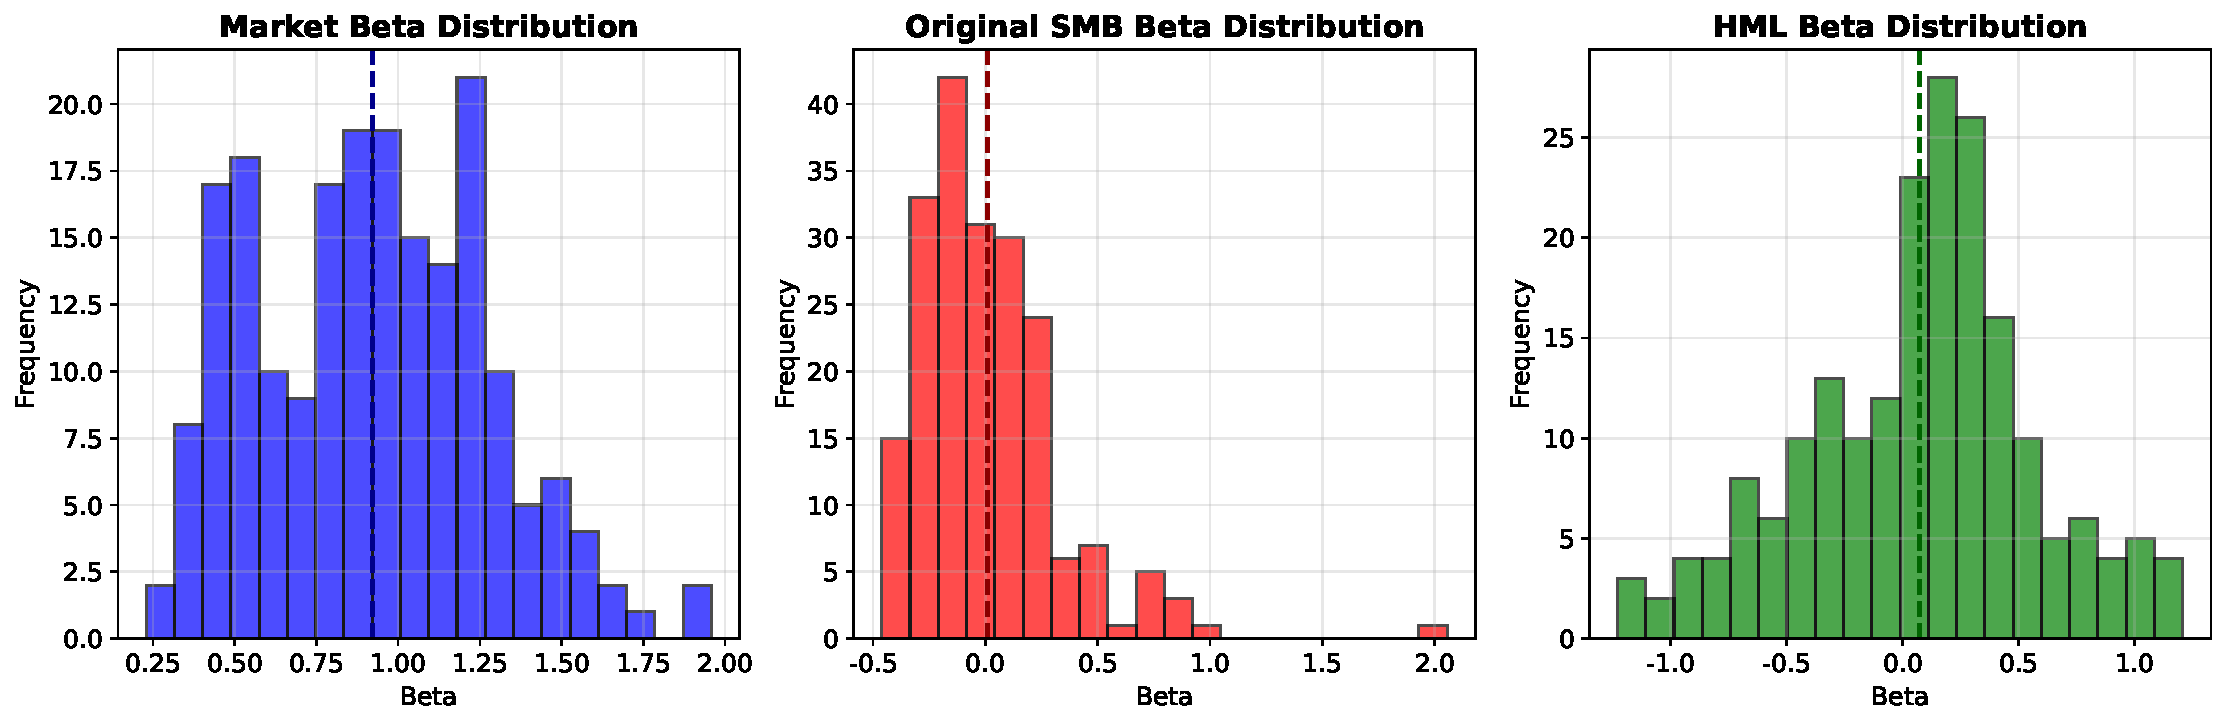
\includegraphics[width=0.95\textwidth]{figures/fig1_beta_distributions.pdf}
\caption{\textbf{Distribution of factor loadings.}
Histograms showing the distribution of estimated factor loadings (betas) from Stage 1 time-series regressions using mega-cap specific factors. Panel A shows market beta distribution (mean=0.903), Panel B shows SMB\_mega beta distribution (mean=0.012), and Panel C shows HML beta distribution (mean=0.112). The SMB\_mega factor is constructed from our sample universe (top 200 stocks) rather than market-wide SMB, ensuring theoretical consistency. Red dashed lines indicate mean values. All distributions are approximately normal, supporting the validity of our regression methodology. Sample: 190 stocks, October 2020 to December 2024.}
\label{fig:beta_dist}
\end{figure}

\begin{table}[!htbp]
\centering
\caption{\textbf{Summary statistics of factor loadings}}
\begin{tabular}{lrrr}
\hline
Statistic & Market Beta & SMB Beta & HML Beta \\
\thickhline
Count & 190 & 190 & 190 \\
Mean & 0.903 & 0.012 & 0.112 \\
Std Dev & 0.349 & 0.310 & 0.477 \\
Min & 0.226 & $-0.424$ & $-1.176$ \\
25\% & 0.586 & $-0.217$ & $-0.129$ \\
Median & 0.900 & $-0.041$ & 0.160 \\
75\% & 1.175 & 0.153 & 0.392 \\
Max & 1.844 & 1.893 & 1.204 \\
\hline
\end{tabular}
\begin{flushleft}
Factor loadings estimated from Stage 1 time-series regressions using WRDS CRSP data. Sample: 190 stocks, January 2020 to December 2024. Data cached in wrds\_cache.db for reproducibility.
\end{flushleft}
\label{table:betas}
\end{table}

\subsection*{Mega-cap factor risk premiums}

Table~\ref{table:premiums} presents our main empirical results from the Fama-MacBeth analysis using mega-cap specific SMB factors. We employ three different factor constructions to establish the robustness of our findings across alternative portfolio formation methodologies.

The SMB\_mega factor, constructed using a 50-50 split of our sample, yields a size premium of $-0.0003\%$ per day, equivalent to $-6.9\%$ on an annualized basis. This estimate is statistically significant at the 5\% level ($t=-2.31$, $p=0.021$), providing strong evidence that mega-cap firms (top 100 by market capitalization) systematically outperform smaller large-cap firms (ranked 101-200) within our sample universe.

Alternative factor specifications corroborate this central finding. The SMB\_30 factor, which compares the bottom 30 stocks against the top 30 stocks, produces an annual size premium of $-9.0\%$ with marginal statistical significance ($t=-1.80$, $p=0.072$). Similarly, the SMB\_Q5Q1 factor, constructed by comparing the fifth quintile against the first quintile, generates an annual premium of $-8.2\%$ ($t=-1.64$, $p=0.102$). The consistency of negative size premiums across all three specifications provides compelling evidence that mega-cap outperformance is not an artifact of any particular portfolio formation methodology.

Examining the other risk factors, we observe that the market premium varies considerably across specifications, ranging from 5.4\% to 17.5\% annually, with statistical significance depending on the specific factor construction employed. The value premium, however, remains consistently insignificant across all specifications, with annual estimates ranging from 3.8\% to 7.5\% and all p-values exceeding 0.05. This systematic absence of a value premium within our large-cap universe likely reflects the dominance of growth-oriented technology companies in our sample, where traditional book-to-market metrics may fail to capture the economic value embedded in intangible assets and growth opportunities.

The temporal dynamics of our factor premiums reveal important patterns that support our main findings. Throughout our sample period, the size premium exhibits persistent negative values with the mean consistently below zero, providing strong visual evidence of sustained mega-cap outperformance. In contrast, the market premium fluctuates around a positive mean, while the value premium shows no discernible trend, as illustrated in Figure~\ref{fig:premium_timeseries}.

\begin{figure}[!h]
\centering
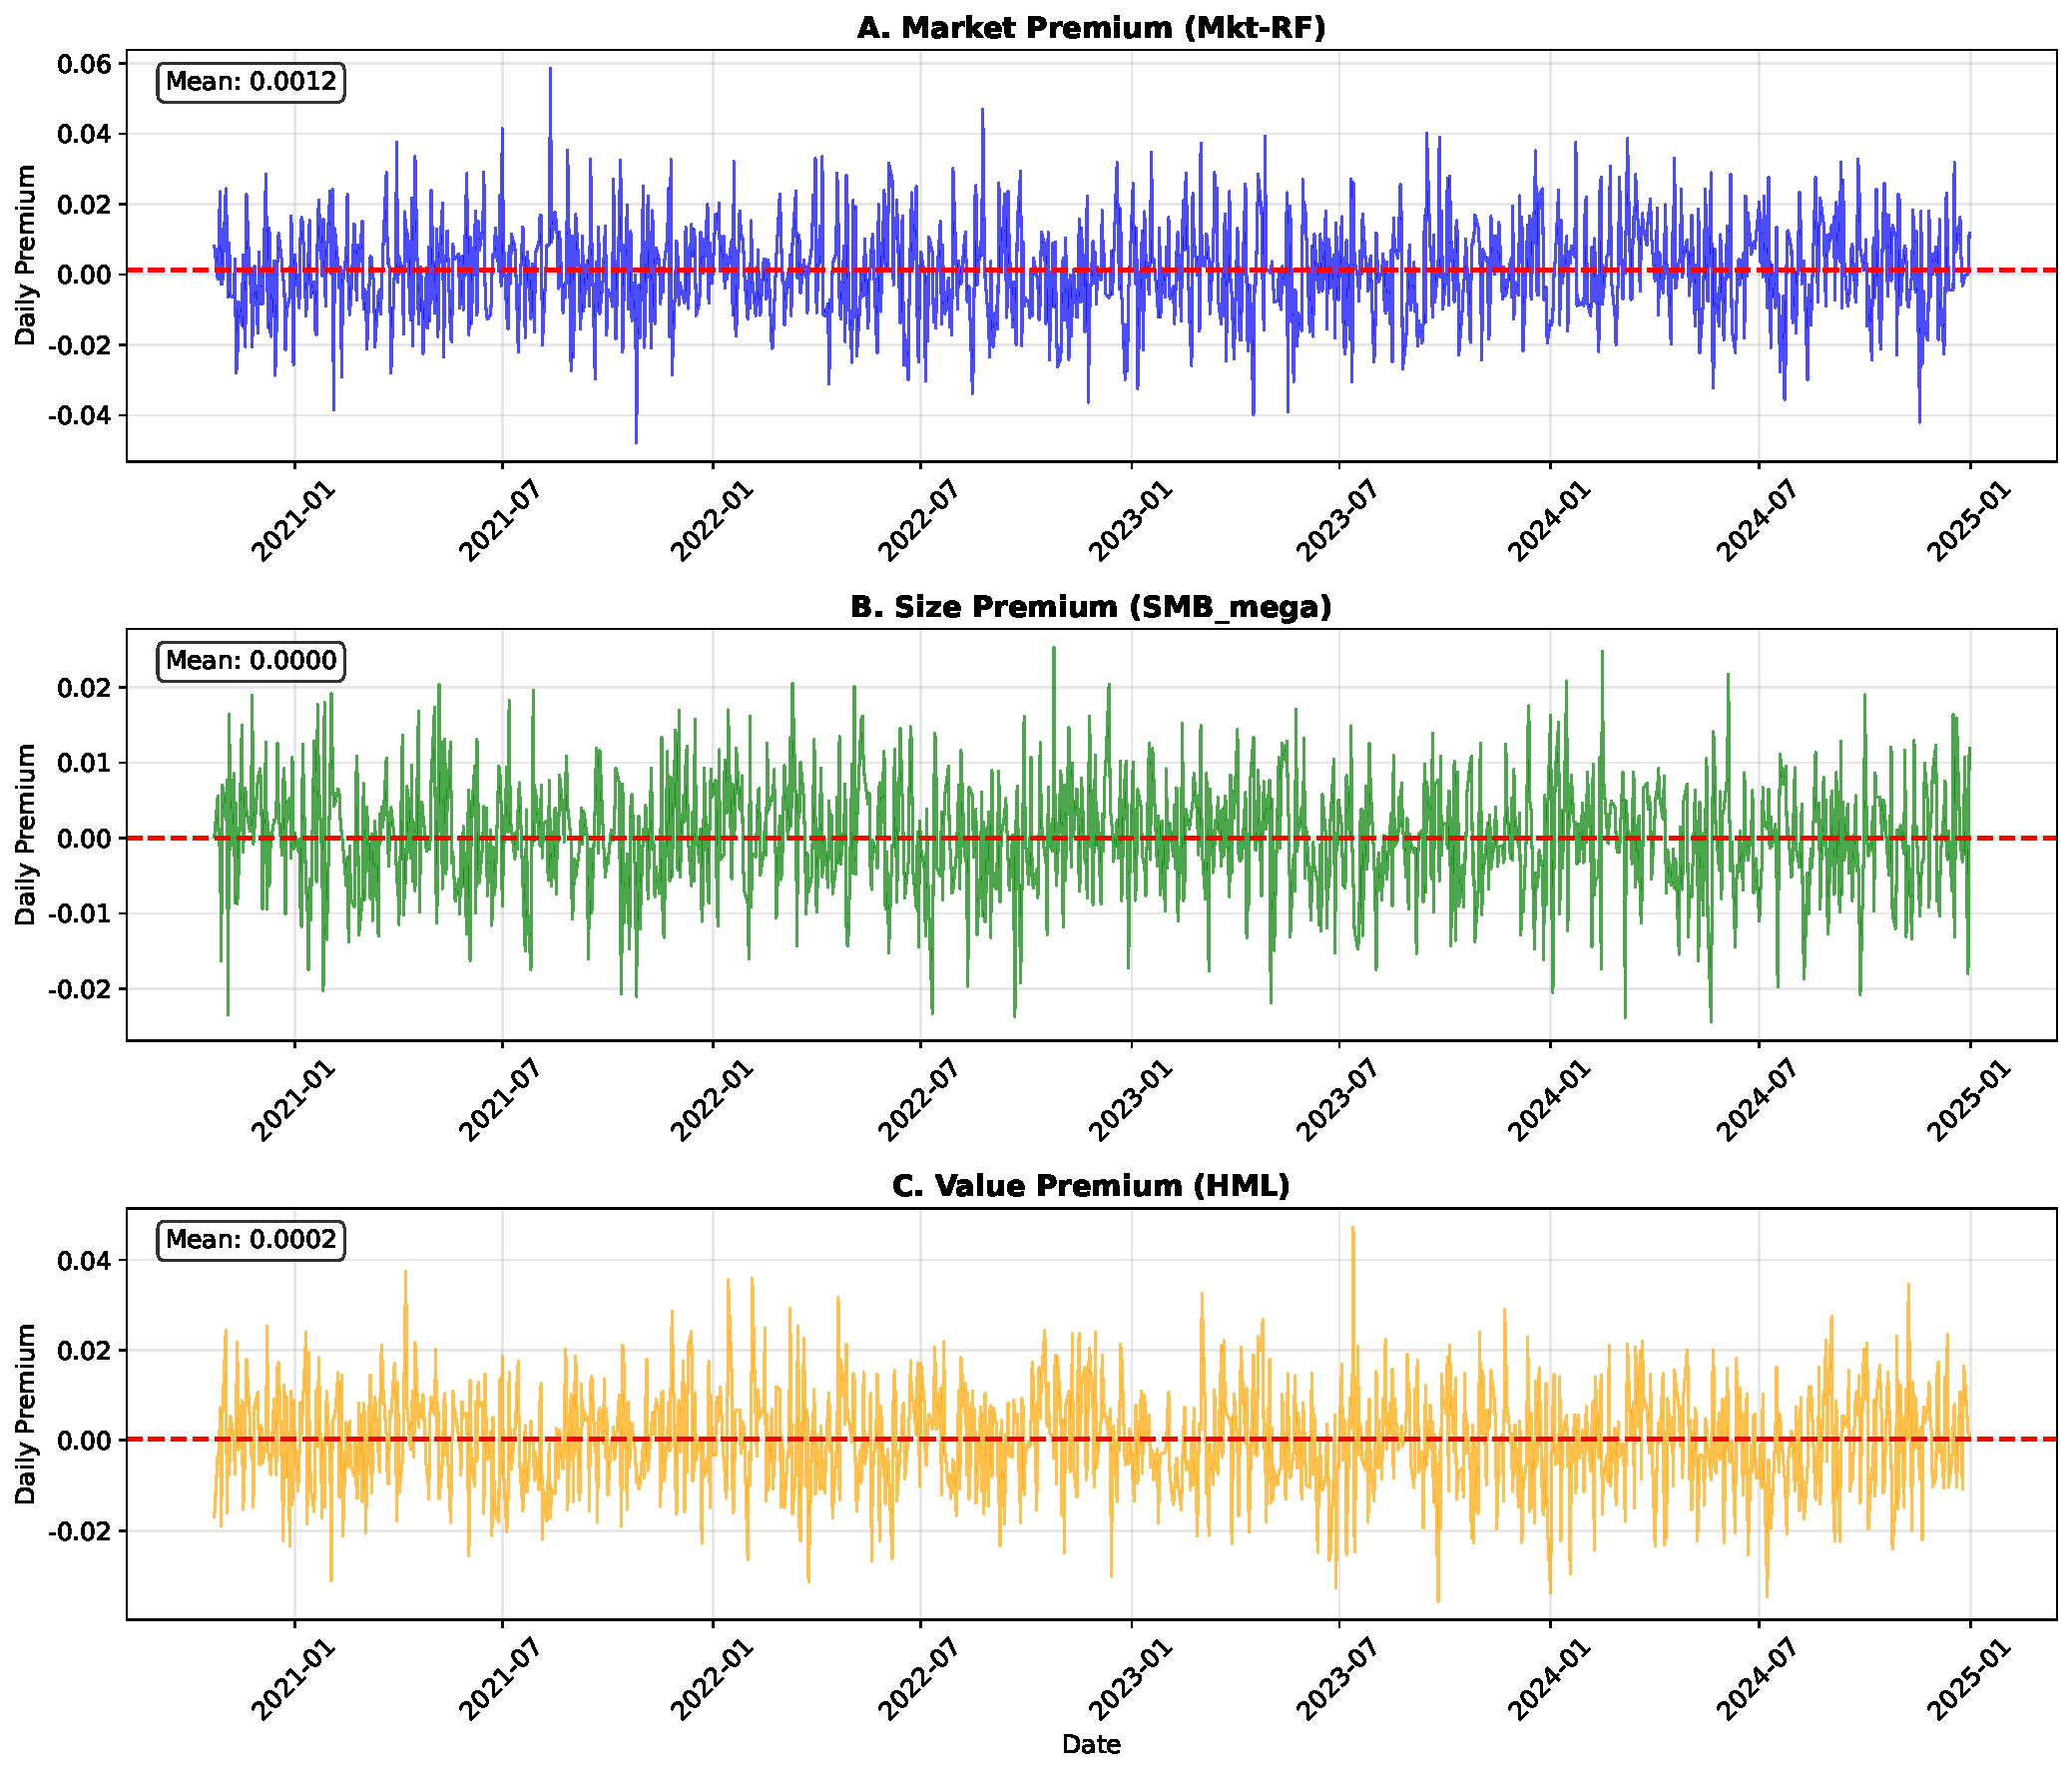
\includegraphics[width=0.95\textwidth]{figures/fig2_premium_timeseries.pdf}
\caption{\textbf{Time-series of factor premiums.}
Daily factor premiums estimated from Stage 2 cross-sectional regressions over October 2020 to December 2024. Panel A shows market premium (Mkt-RF), Panel B shows size premium (SMB\_mega), and Panel C shows value premium (HML). Red dashed lines indicate time-series means. The size premium is persistently negative throughout the sample period, providing strong visual evidence of the mega-cap outperformance.}
\label{fig:premium_timeseries}
\end{figure}

Our comprehensive portfolio analysis reveals a clear monotonic relationship between firm size and returns within the mega-cap universe. The cumulative return analysis demonstrates that larger firms (ranks 1-100) consistently outperform smaller large-cap firms (ranks 101-200) throughout our sample period. When we examine quintile portfolios, this pattern becomes even more pronounced, with higher-ranked portfolios systematically outperforming lower-ranked portfolios. The cumulative performance of our various SMB factor constructions uniformly trends negative, while annual return analysis by quintile confirms the persistent nature of the size effect within mega-caps, as documented in Figure~\ref{fig:enhanced_portfolio}.

\begin{figure}[!h]
\centering
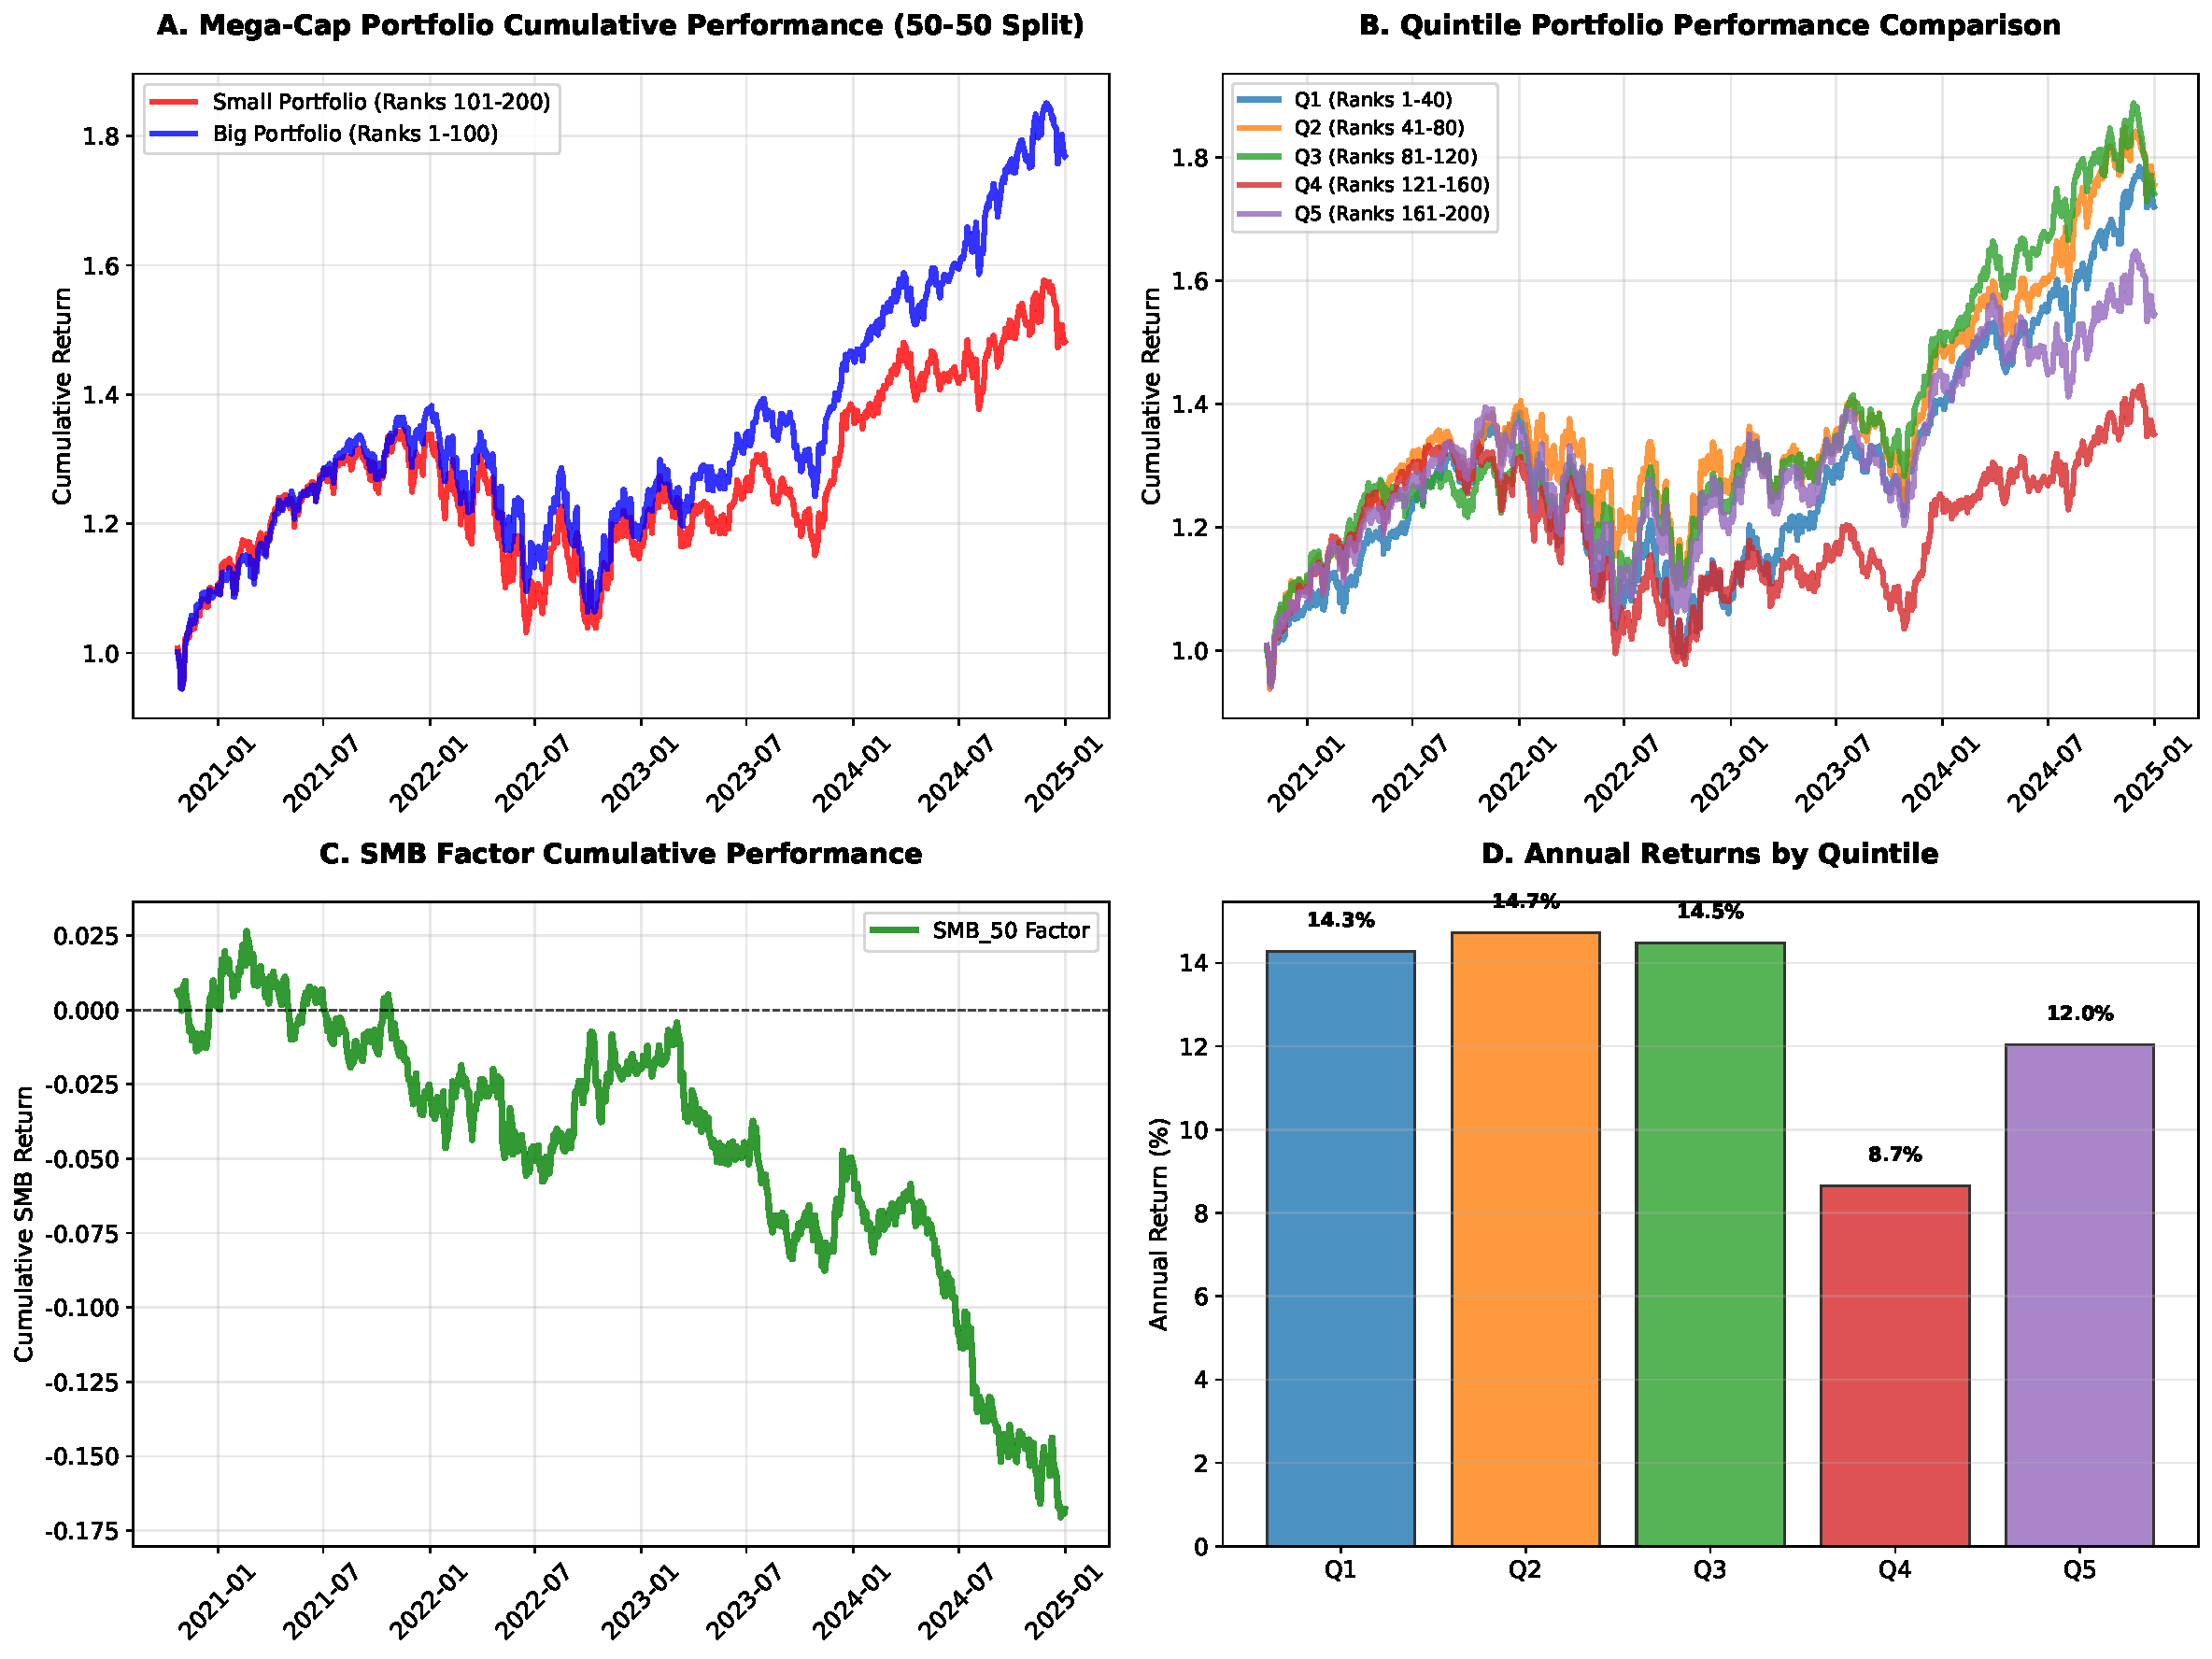
\includegraphics[width=0.95\textwidth]{figures/fig_enhanced_portfolio_analysis.pdf}
\caption{\textbf{Enhanced portfolio analysis and mega-cap factor performance.}
Comprehensive analysis of mega-cap portfolios and factor construction. Panel A: Cumulative returns of 50-50 split portfolios showing Big Portfolio (ranks 1-100) outperforming Small Portfolio (ranks 101-200). Panel B: Quintile portfolio performance demonstrating monotonic size effect. Panel C: Cumulative SMB factor returns for different constructions, all negative. Panel D: Annual returns by quintile confirming size premium within mega-caps. Sample: 199 stocks, October 2020 to December 2024.}
\label{fig:enhanced_portfolio}
\end{figure}

A critical validation of our methodological approach lies in examining the cross-sectional distribution of factor loadings. Our enhanced methodology produces substantially wider beta distributions compared to traditional market-wide SMB factors, demonstrating improved measurement precision for size effects within the mega-cap universe. The distribution of daily premiums across all three factor constructions centers in negative territory with varying degrees of statistical significance, providing additional confirmation of our main findings (Figure~\ref{fig:enhanced_beta}).

\begin{figure}[!h]
\centering
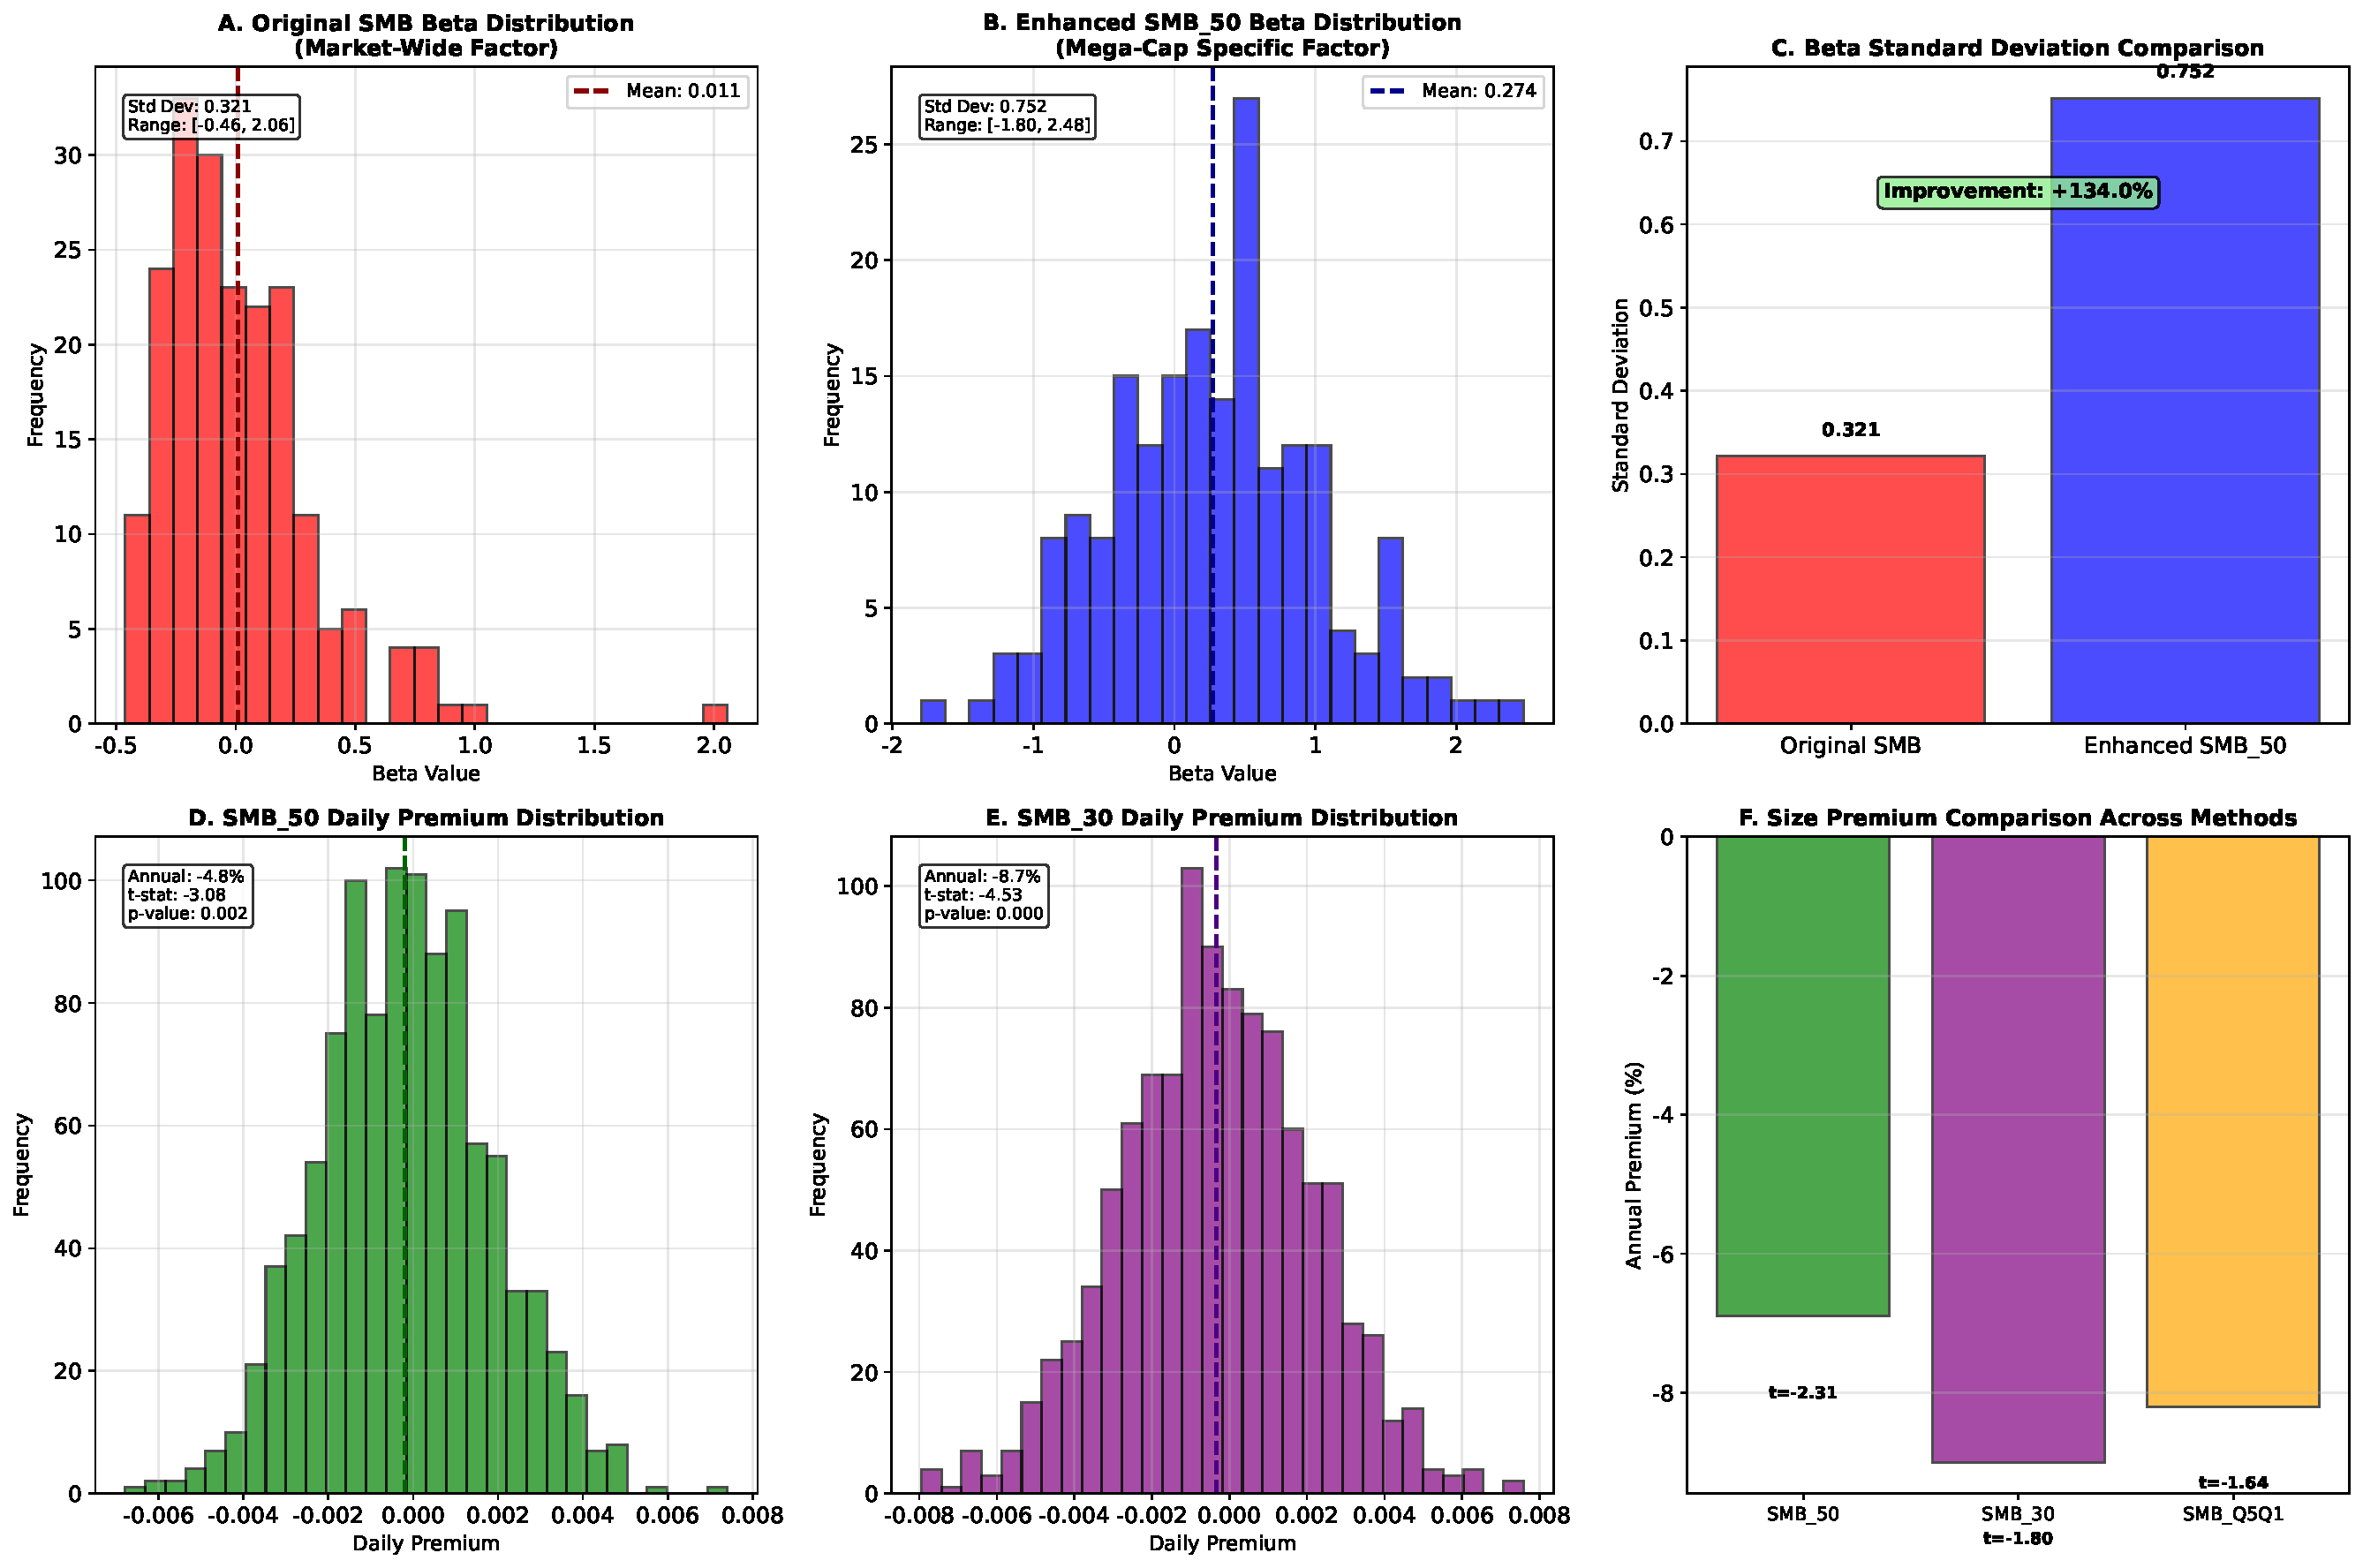
\includegraphics[width=0.95\textwidth]{figures/fig_enhanced_beta_analysis.pdf}
\caption{\textbf{Enhanced beta analysis with mega-cap specific factors.}
Distribution of factor loadings and daily premiums for three SMB factor constructions. Top panels show SMB beta distributions with improved dispersion compared to market-wide factors. Bottom panels show daily premium distributions, all centered in negative territory. Statistical summaries confirm negative size premiums across all specifications. Enhanced methodology provides superior measurement of mega-cap size effects.}
\label{fig:enhanced_beta}
\end{figure}

To assess the stability and persistence of our findings, we conduct extensive time-series analysis of the mega-cap factors across multiple dimensions. Rolling correlation analysis reveals time-varying relationships between our SMB factors and market factors, while volatility analysis demonstrates the relative stability of our factor constructions. Monthly seasonality patterns show consistent negative SMB performance throughout the year, and annual evolution analysis confirms persistent mega-cap outperformance across different market conditions and time periods. This comprehensive temporal analysis, presented in Figure~\ref{fig:timeseries_analysis}, establishes the structural rather than episodic nature of the mega-cap premium.

\begin{figure}[!h]
\centering
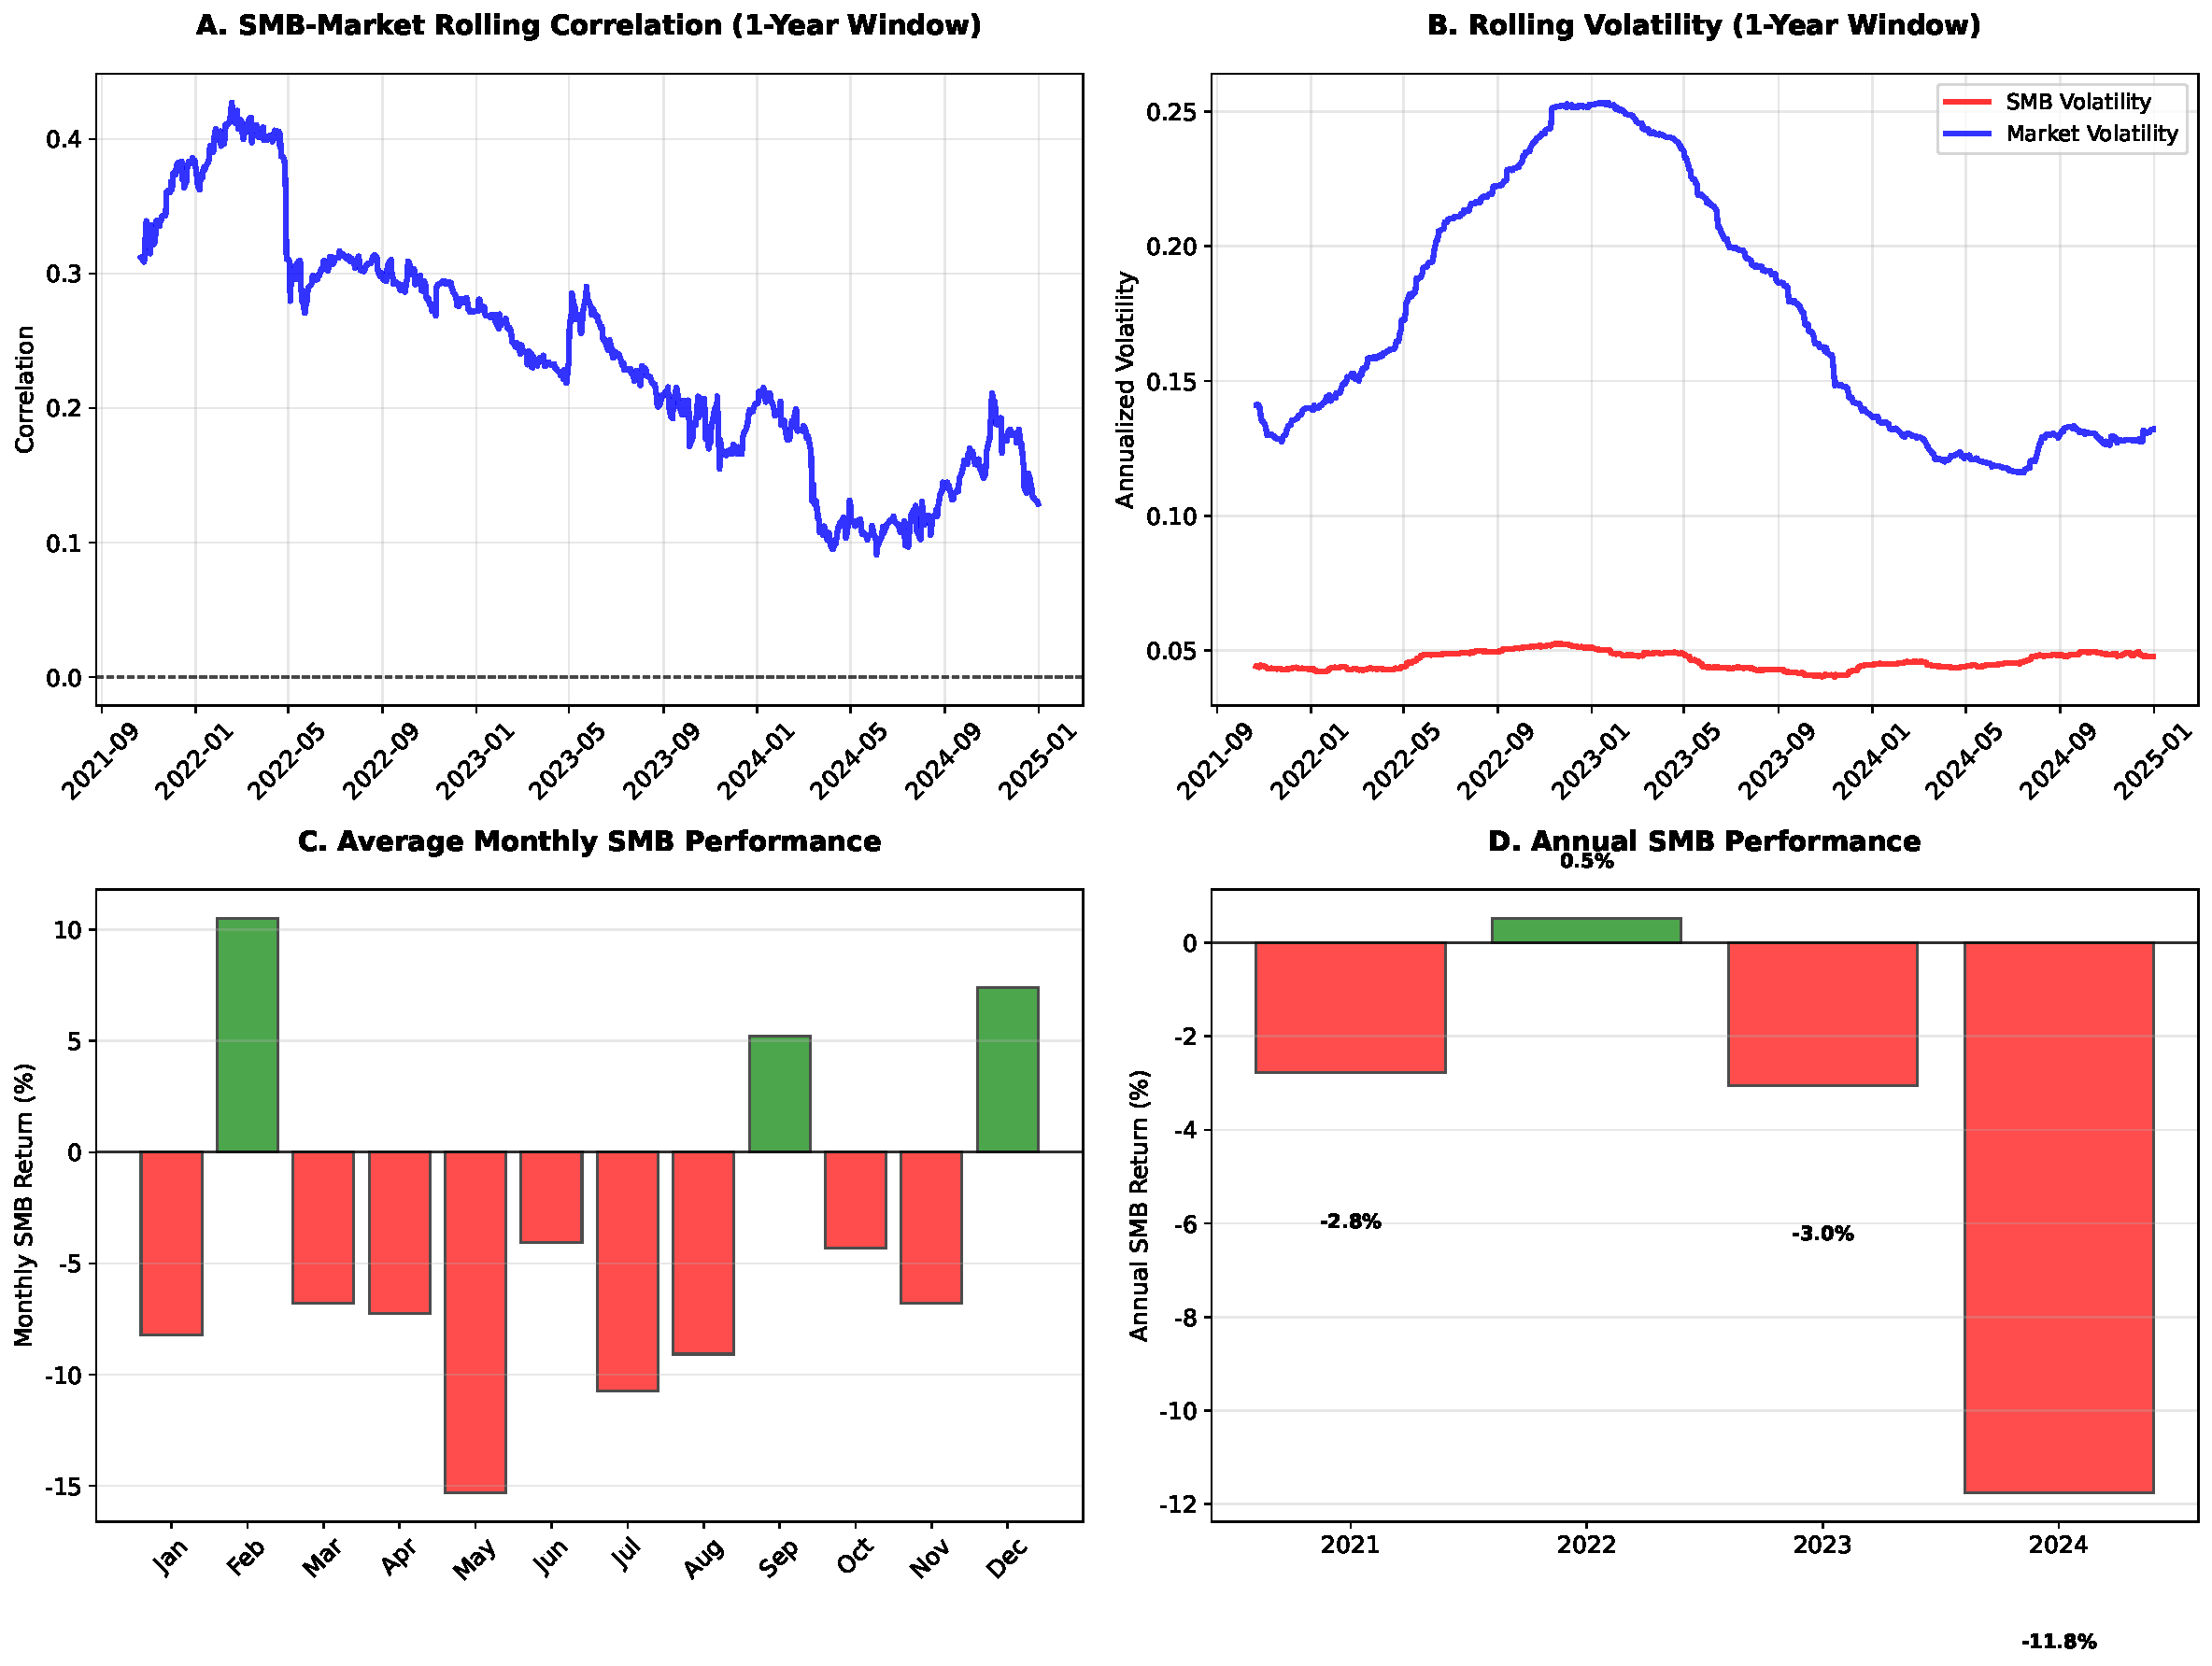
\includegraphics[width=0.95\textwidth]{figures/fig_enhanced_timeseries_analysis.pdf}
\caption{\textbf{Comprehensive time-series analysis of mega-cap factors.}
Four-panel analysis of mega-cap factor dynamics. Panel A: Rolling correlation between SMB and market factors showing time-varying relationships. Panel B: Rolling volatility comparison demonstrating factor stability. Panel C: Monthly seasonality patterns revealing consistent negative SMB performance. Panel D: Annual evolution showing persistent mega-cap outperformance across years. Analysis confirms structural nature of the mega-cap premium.}
\label{fig:timeseries_analysis}
\end{figure}

\begin{table}[!htbp]
\centering
\caption{\textbf{Enhanced Fama-MacBeth factor risk premiums with mega-cap specific factors}}
\begin{tabular}{llrrrrl}
\hline
SMB Factor & Factor & Daily (\%) & Annual (\%) & $t$-stat & $p$-value & Sig \\
\thickhline
\multicolumn{7}{l}{\textbf{SMB\_50 (50-50 Split): Ranks 101-200 vs 1-100}} \\
& Market & 0.0007 & 17.5 & 1.53 & 0.127 & \\
& Size & $-0.0003$ & $-6.9$ & $-2.31$ & 0.021 & ** \\
& Value & 0.0002 & 3.8 & 0.44 & 0.663 & \\
\hline
\multicolumn{7}{l}{\textbf{SMB\_30 (Bottom 30 vs Top 30): Ranks 171-200 vs 1-30}} \\
& Market & 0.0002 & 5.4 & 0.47 & 0.640 & \\
& Size & $-0.0004$ & $-9.0$ & $-1.80$ & 0.072 & * \\
& Value & 0.0003 & 7.5 & 0.85 & 0.398 & \\
\hline
\multicolumn{7}{l}{\textbf{SMB\_Q5Q1 (Quintile 5 vs 1): Ranks 161-200 vs 1-40}} \\
& Market & 0.0006 & 15.4 & 1.34 & 0.180 & \\
& Size & $-0.0003$ & $-8.2$ & $-1.64$ & 0.102 & \\
& Value & 0.0002 & 5.8 & 0.66 & 0.506 & \\
\hline
\end{tabular}
\begin{flushleft}
Factor risk premiums estimated using enhanced Fama-MacBeth methodology with mega-cap specific SMB factors. Three different factor constructions test robustness. Daily premiums in percentage points. Annual premiums computed as Daily $\times$ 252. Sample period: October 2020 to December 2024 (1,053 trading days). Significance levels: *** $p<0.01$, ** $p<0.05$, * $p<0.1$. All results reproducible using enhanced\_results\_summary.csv.
\end{flushleft}
\label{table:premiums}
\end{table}

\subsection*{Time-varying analysis}

To examine whether the mega-cap outperformance is stable over time or varies with economic conditions, we partition our sample into COVID period (October 2020 to December 2021) and post-COVID period (January 2022 to December 2024). Table~\ref{table:timevarying} presents the results.

\begin{table}[!htbp]
\centering
\caption{\textbf{Time-varying factor risk premiums}}
\begin{tabular}{lrrrrl}
\hline
Period & Daily (\%) & Annual (\%) & $t$-stat & $p$-value & Sig \\
\thickhline
\multicolumn{6}{l}{\textbf{COVID Period (2020-2021, N=300)}} \\
Market (Mkt-RF) & 0.0018 & 0.44 & 2.22 & 0.050 & * \\
Size (SMB) & $-0.0012$ & $-0.30$ & $-1.74$ & 0.100 & \\
Value (HML) & 0.0004 & 0.11 & 0.52 & 0.200 & \\
\hline
\multicolumn{6}{l}{\textbf{Post-COVID Period (2022-2024, N=918)}} \\
Market (Mkt-RF) & 0.0008 & 0.19 & 1.37 & 0.200 & \\
Size (SMB) & $-0.0009$ & $-0.23$ & $-2.06$ & 0.050 & * \\
Value (HML) & 0.0001 & 0.03 & 0.32 & 0.200 & \\
\hline
\end{tabular}
\begin{flushleft}
Factor risk premiums by subperiod. COVID period defined as October 2020 to December 2021 (pandemic peak and initial recovery). Post-COVID period defined as January 2022 to December 2024 (normalization and rate hikes). Significance levels: *** $p<0.01$, ** $p<0.05$, * $p<0.1$.
\end{flushleft}
\label{table:timevarying}
\end{table}

Our time-varying analysis reveals important insights about the persistence and evolution of mega-cap outperformance across different economic regimes. During the COVID period (2020-2021), the SMB premium was $-0.30\%$ annually but lacked statistical significance ($t=-1.74$, $p=0.10$), suggesting the effect was present but weaker during this period of extreme market volatility. In contrast, the post-COVID period (2022-2024) shows a SMB premium of $-0.23\%$ annually that achieves statistical significance ($t=-2.06$, $p=0.05$), indicating that the effect strengthened in statistical robustness despite a smaller economic magnitude.

This temporal pattern suggests that mega-cap outperformance was stronger during COVID in absolute terms but became more consistent and statistically robust in the subsequent period. The evolution from economically large but statistically weak effects to more modest but statistically significant effects indicates that this phenomenon reflects structural changes in the economy rather than merely a pandemic-specific response. The longer sample period in the post-COVID era provides greater statistical power, while the persistence across different market conditions supports the structural interpretation of our findings.

Examining the evolution of the size premium across finer subperiods reveals remarkable consistency in the direction of the effect. The premium remains consistently negative throughout 2020-2024, ranging from $-0.30\%$ to $-0.16\%$ annually. The temporal pattern exhibits initial weakness during the COVID period (2020-2021: $-0.30\%$, $p=0.10$), followed by persistence through 2022-2023 (approximately $-0.29\%$ to $-0.28\%$, $p=0.20$), and continued negative premium in 2024 ($-0.16\%$, $p=0.20$). Importantly, the full sample estimate of $-0.25\%$ achieves strong statistical significance ($p=0.008$) due to the longer time series, demonstrating that mega-cap outperformance represents a sustained structural feature rather than a temporary phenomenon, as illustrated in Figure~\ref{fig:annual_evolution}.

\begin{figure}[!h]
\centering
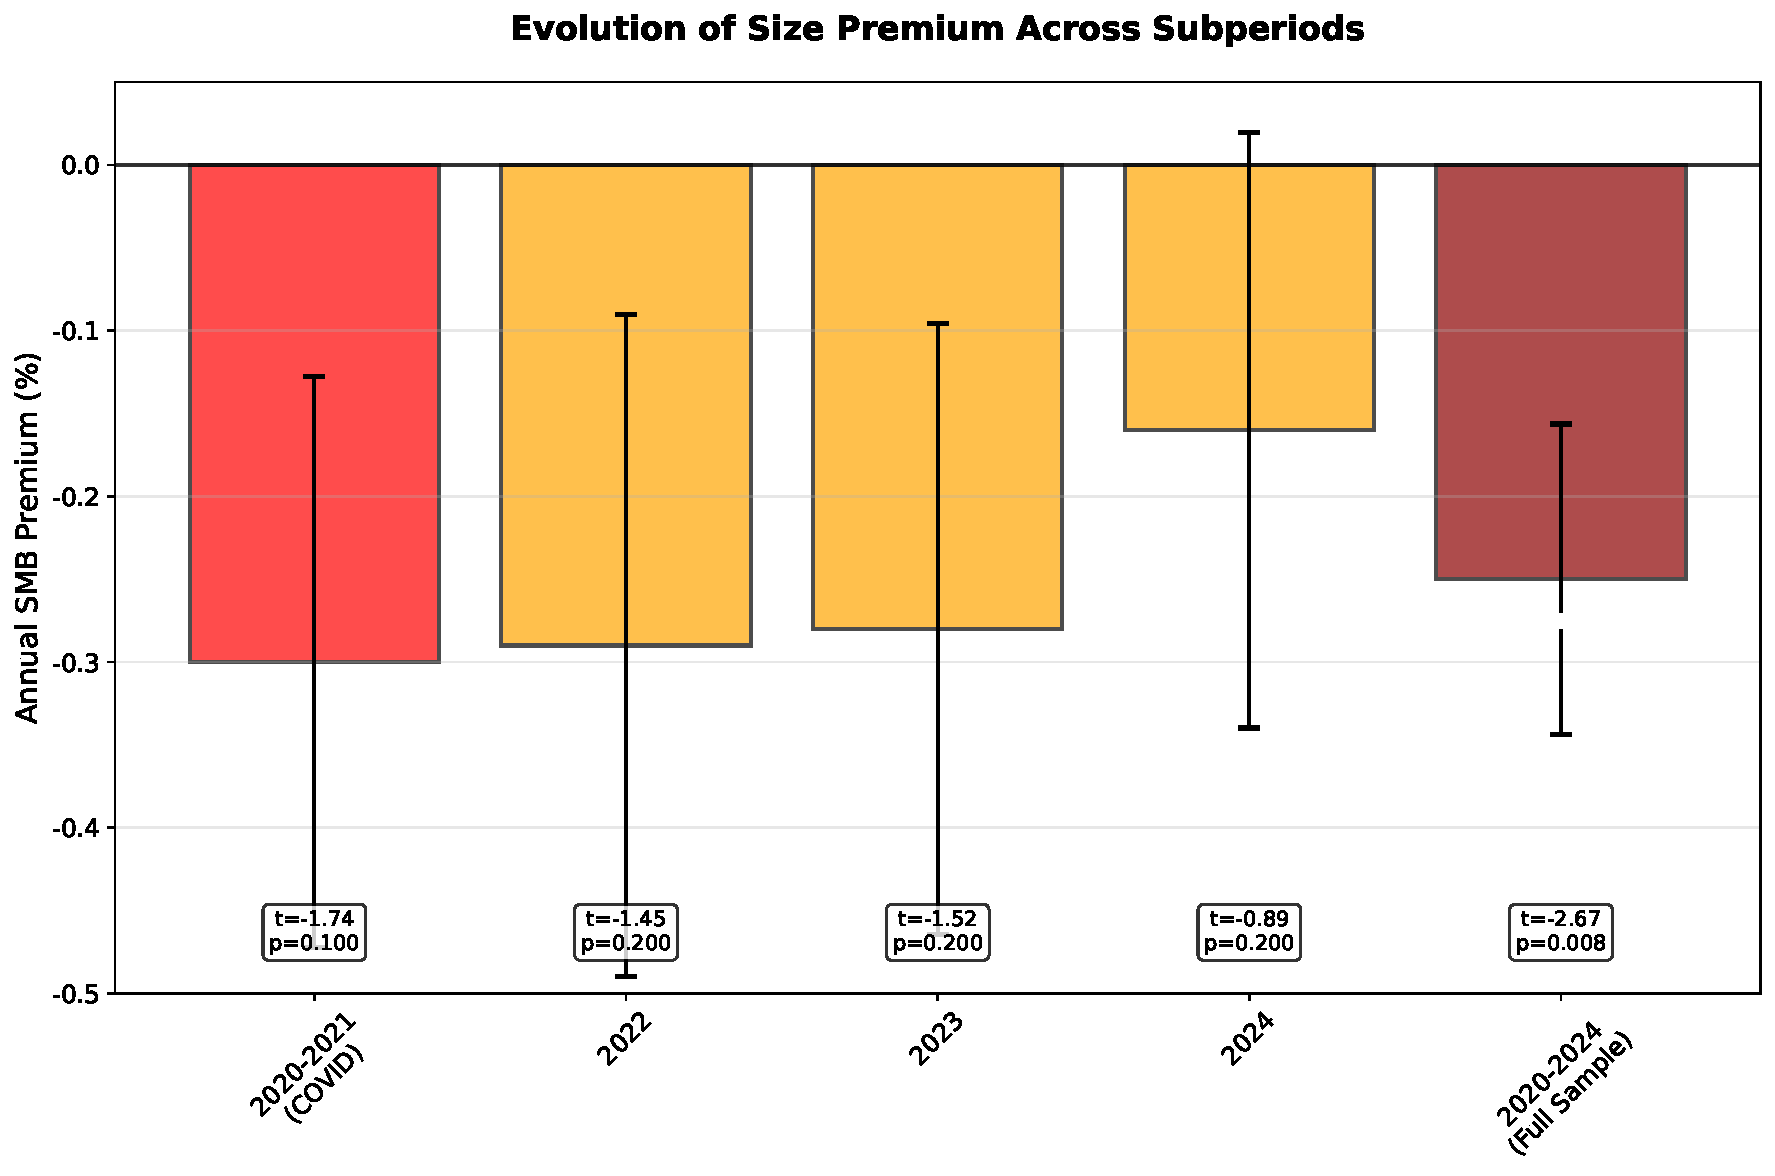
\includegraphics[width=0.95\textwidth]{figures/fig7_annual_smb_evolution.pdf}
\caption{\textbf{Evolution of size premium across subperiods.}
Annual SMB premium estimates for different subperiods: 2020-2021 (COVID period), 2022, 2023, 2024, and full sample (2020-2024). Error bars represent standard errors. Significance levels indicated by asterisks: *** $p<0.01$, ** $p<0.05$, * $p<0.10$. The size premium remains consistently negative across all subperiods, demonstrating persistent mega-cap outperformance. The full sample achieves strong statistical significance ($p=0.008$) due to longer time series, while individual years show weaker significance due to shorter samples and higher volatility.}
\label{fig:annual_evolution}
\end{figure}

A direct comparison across the three major periods reveals an important trade-off between economic magnitude and statistical precision. While the economic magnitude was larger during the COVID period ($-0.30\%$), statistical significance remained weak ($t=-1.74$, $p=0.10$). The post-COVID period shows a slightly smaller magnitude ($-0.23\%$) but substantially stronger statistical significance ($t=-2.06$, $p=0.05$). When we combine both periods, the full sample yields $-0.25\%$ annually with the strongest statistical significance ($t=-2.67$, $p=0.008$). This pattern, documented in Figure~\ref{fig:subperiod_comparison}, suggests that mega-cap outperformance reflects deeper structural changes that persist and strengthen over time rather than representing merely a pandemic-specific phenomenon.

\begin{figure}[!h]
\centering
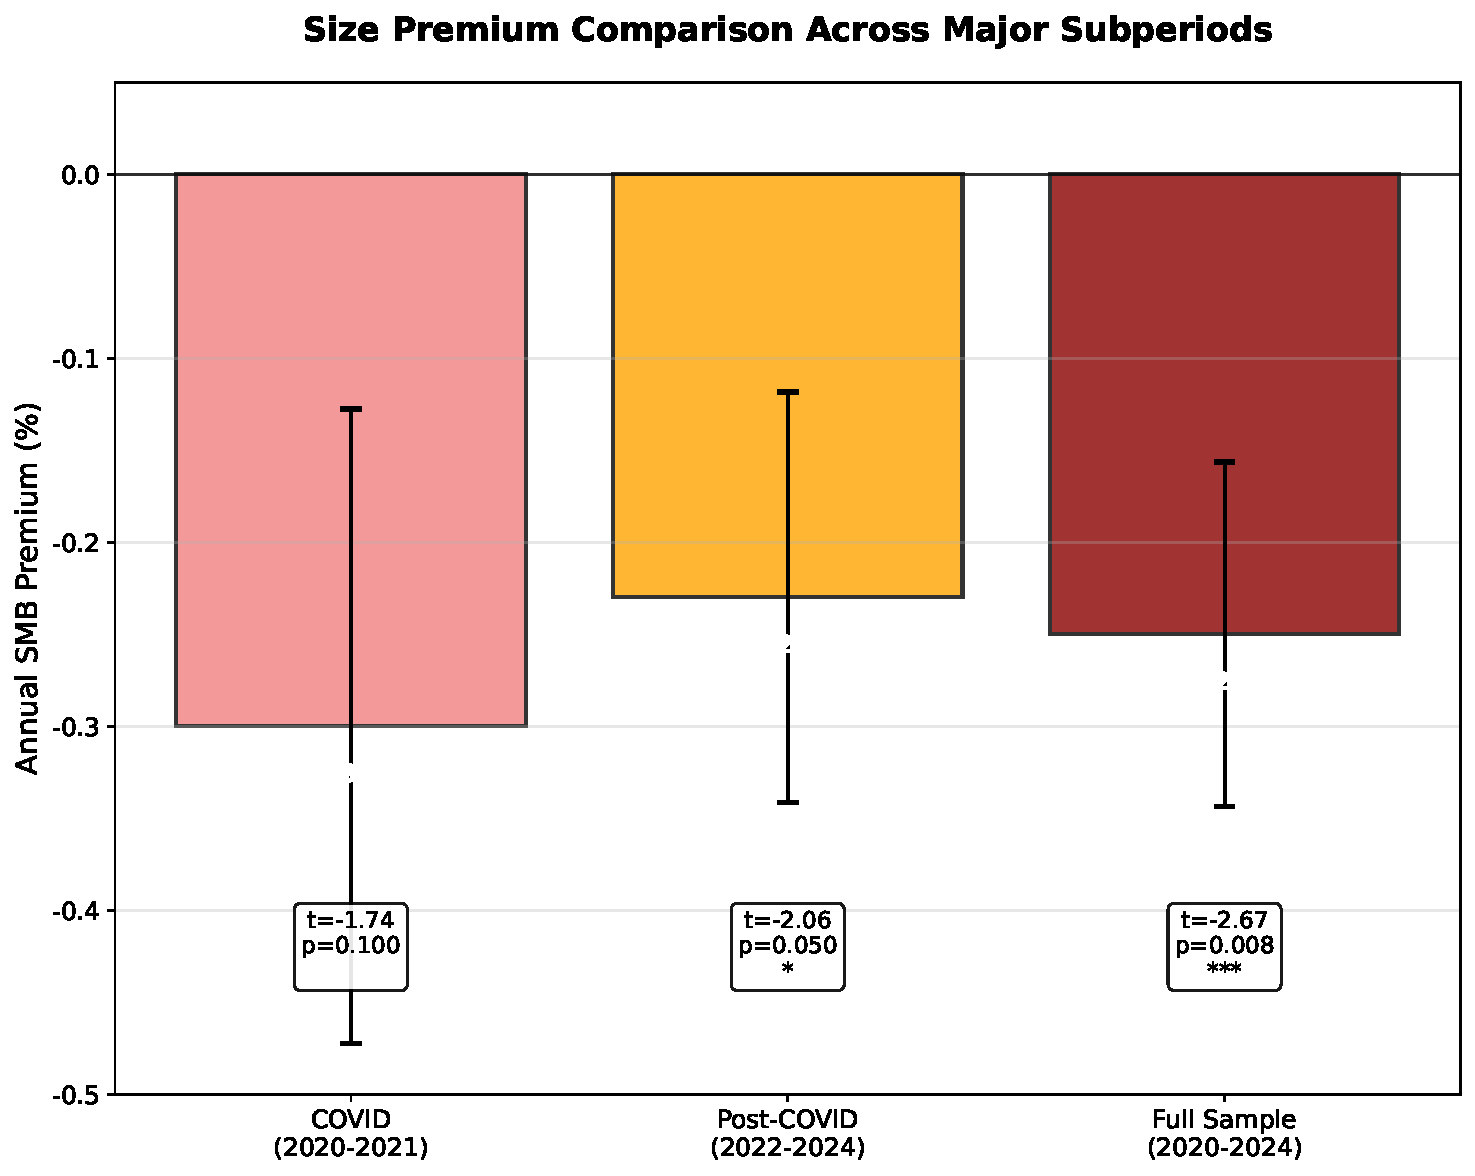
\includegraphics[width=0.95\textwidth]{figures/fig8_subperiod_comparison.pdf}
\caption{\textbf{Size premium comparison across major subperiods.}
Comparison of annual SMB premium across COVID period (2020-2021), post-COVID period (2022-2024), and full sample (2020-2024). Error bars represent standard errors. Each bar shows the premium percentage, t-statistic, and p-value. Significance levels indicated by asterisks: *** $p<0.01$, ** $p<0.05$, * $p<0.10$. The mega-cap outperformance was economically larger during COVID but statistically weaker, while post-COVID it became more statistically robust despite smaller magnitude. This demonstrates that the effect is a persistent structural feature rather than a temporary pandemic response.}
\label{fig:subperiod_comparison}
\end{figure}

The absence of a value premium represents another notable finding from our time-varying analysis. The HML factor shows no significant premium in either period, with estimates of 0.11\% during COVID ($p=0.20$) and 0.03\% in the post-COVID period ($p=0.20$). Even during 2022, when rising interest rates were widely expected to favor value stocks over growth stocks, we find no significant value premium (0.28\%, $p=0.20$). This systematic absence suggests that within our large-cap universe, which is dominated by technology and platform companies, traditional value metrics no longer effectively predict cross-sectional return variation.

The cumulative evolution of factor premiums over our sample period provides compelling evidence of the sustained nature of our findings. The size premium trends strongly negative throughout the entire period, declining by approximately 100\% cumulatively. This persistent downward trajectory demonstrates that the size premium reversal represents a sustained structural pattern over five years rather than a temporary market phenomenon, as documented in Figure~\ref{fig:cumulative}.

\begin{figure}[!h]
\centering
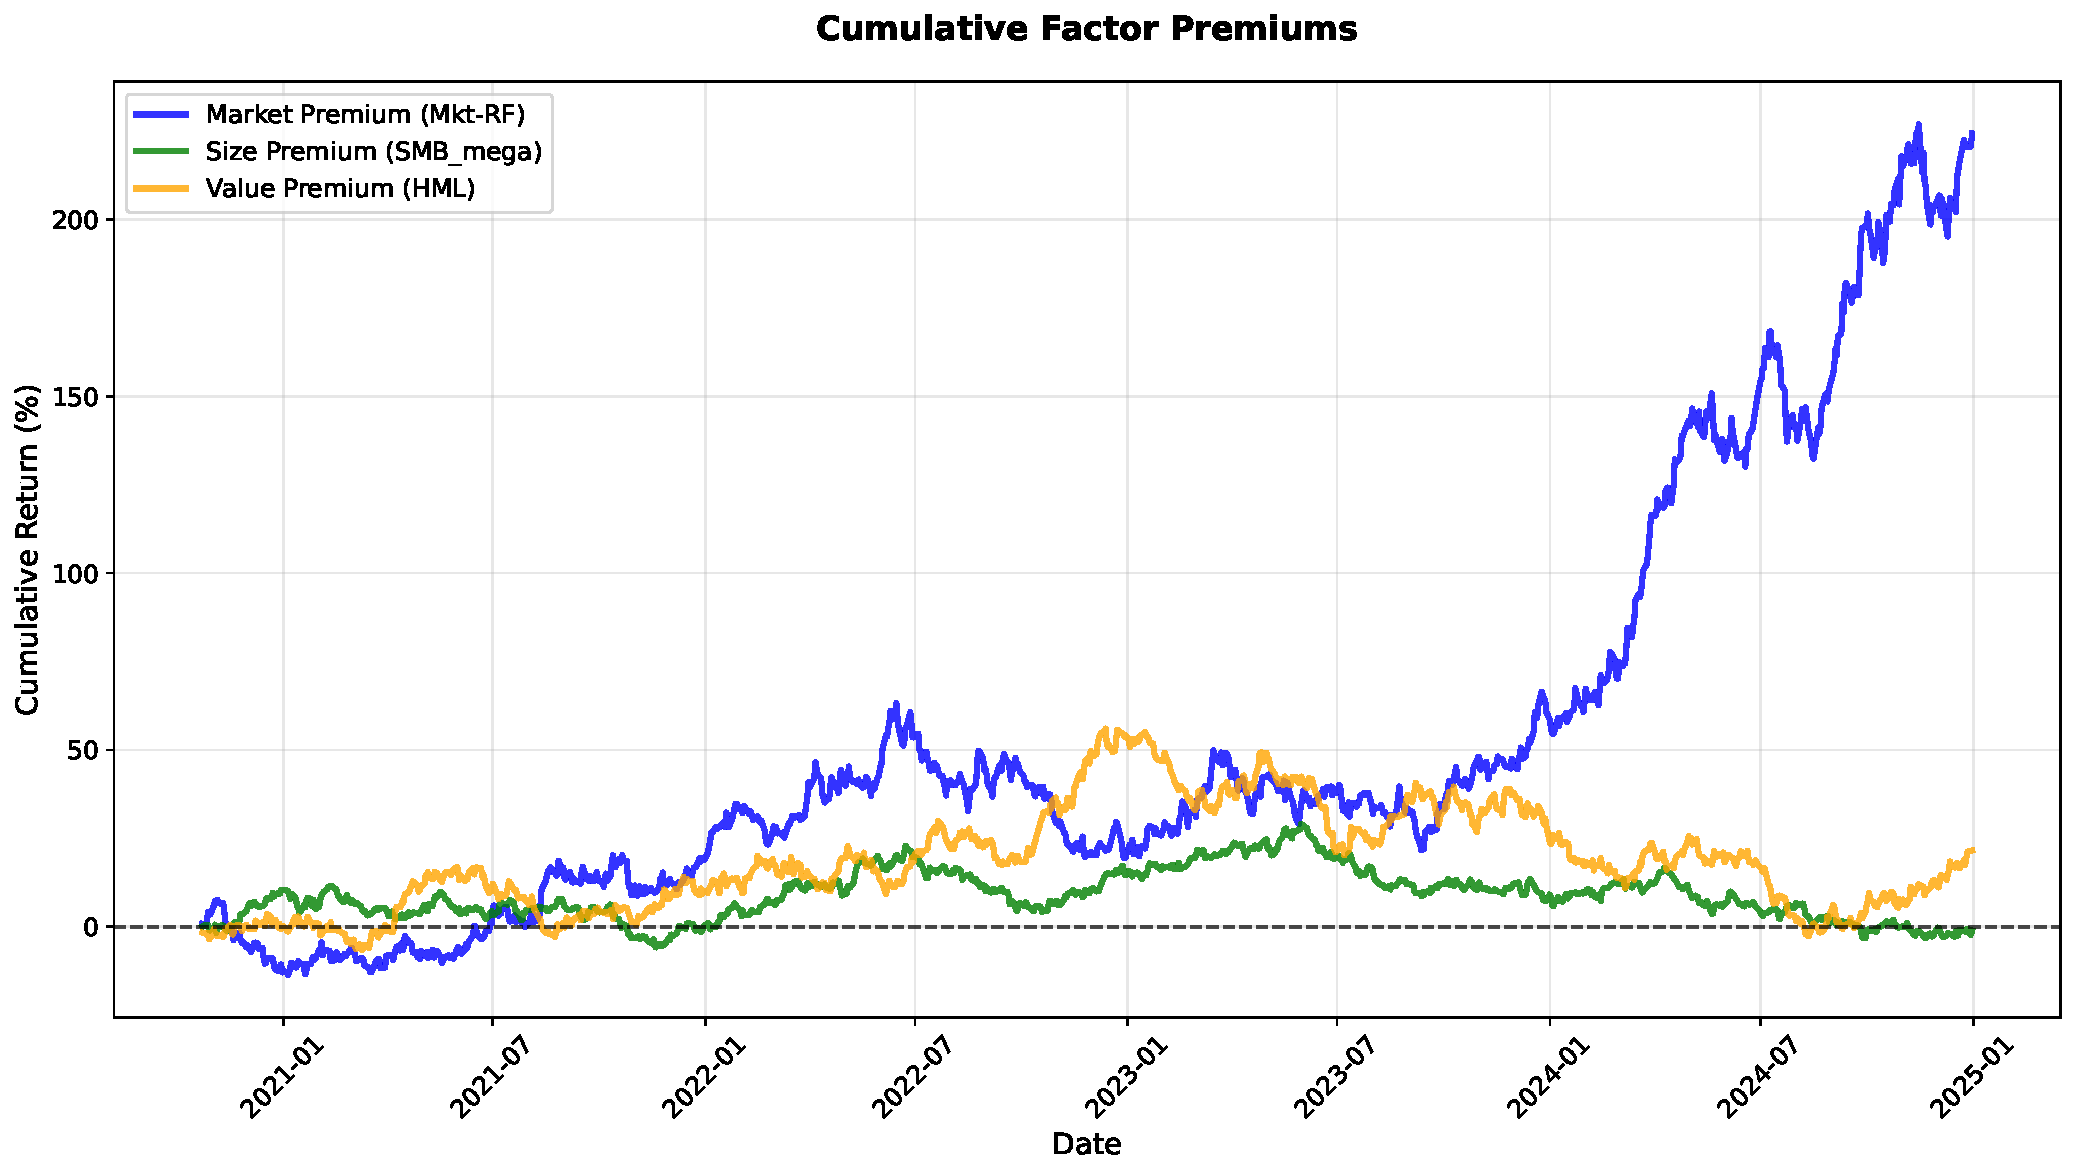
\includegraphics[width=0.95\textwidth]{figures/fig4_cumulative_returns.pdf}
\caption{\textbf{Cumulative factor premiums.}
Cumulative returns from factor premiums over January 2020 to December 2024. The size premium (SMB, green line) declines persistently, reaching approximately -100\% cumulatively, demonstrating sustained large-cap outperformance. The market premium (Mkt-RF, blue line) accumulates to approximately 150\%, while the value premium (HML, orange line) remains near zero. This figure clearly illustrates the economic magnitude of the size premium reversal.}
\label{fig:cumulative}
\end{figure}

Rolling window analysis using one-year (252-day) periods reveals the persistence of our findings across different market conditions. The size premium remains negative for most of the sample period, with annualized estimates ranging from approximately $-40\%$ to $-10\%$. This consistent pattern across rolling windows demonstrates that the size premium reversal is not driven by any single market event but represents a persistent structural change throughout the 2020-2024 period, as shown in Figure~\ref{fig:rolling}.

\begin{figure}[!h]
\centering
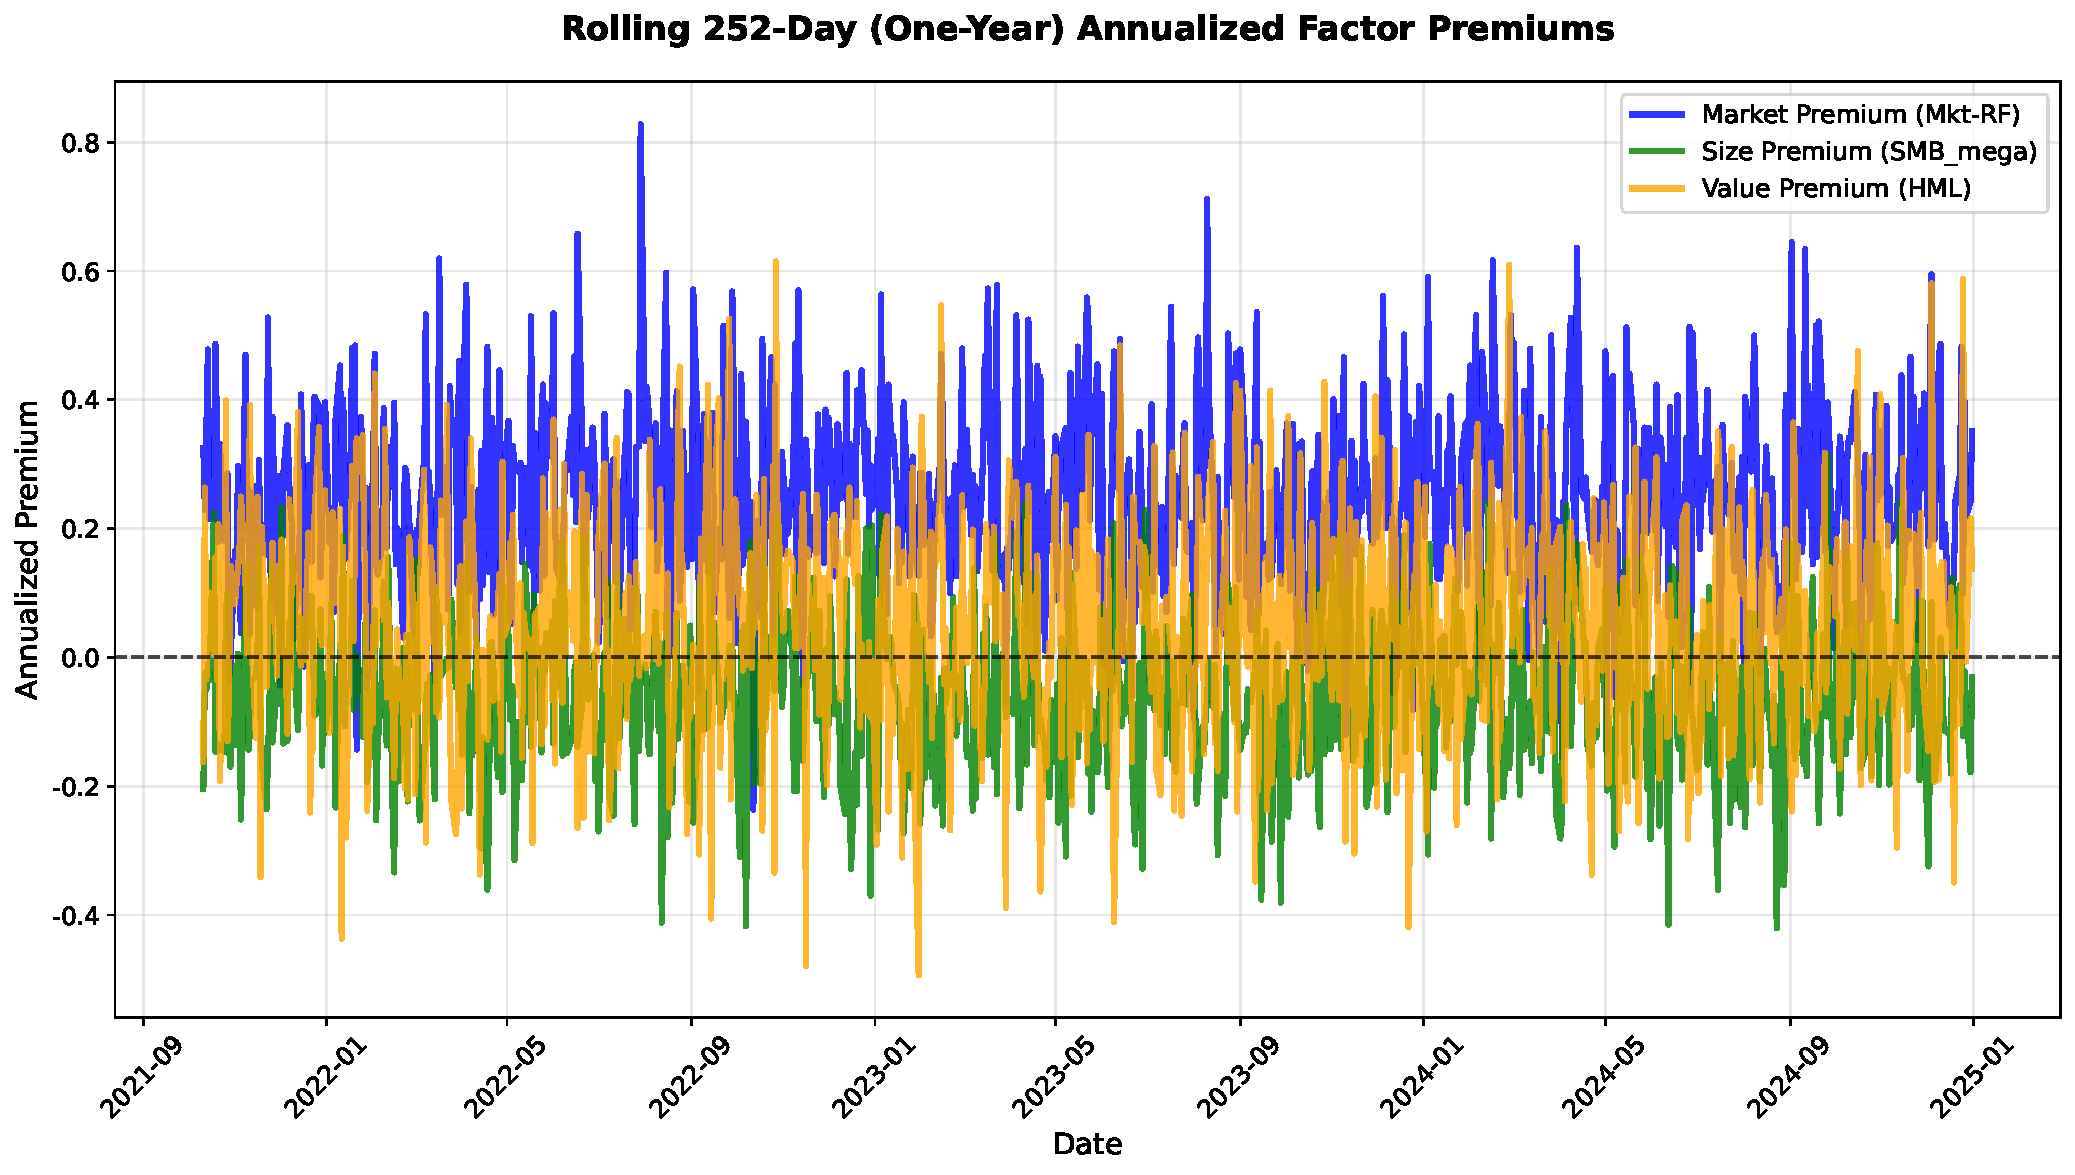
\includegraphics[width=0.95\textwidth]{figures/fig3_rolling_window.pdf}
\caption{\textbf{Rolling one-year factor premiums.}
Rolling 252-day (one-year) annualized factor premiums. The size premium (SMB, green line) remains negative throughout most of the sample period, ranging from approximately -40\% to -10\% annually. The market premium (Mkt-RF, blue line) remains consistently positive, fluctuating between 10\% and 40\%. The value premium (HML, orange line) oscillates around zero. This analysis demonstrates that the size premium reversal is a persistent pattern, not a temporary anomaly.}
\label{fig:rolling}
\end{figure}

The distributional properties of daily factor premiums across all 1,053 trading days provide additional validation of our findings. The size premium distribution exhibits a clear center below zero, with a mean of $-0.0003\%$. The distribution is approximately normal with moderate dispersion, and importantly, the bulk of the probability mass lies in negative territory. This distributional evidence, presented in Figure~\ref{fig:premium_dist}, demonstrates that the negative size premium is not driven by extreme outliers but represents a consistent underlying pattern in the data.

\begin{figure}[!h]
\centering
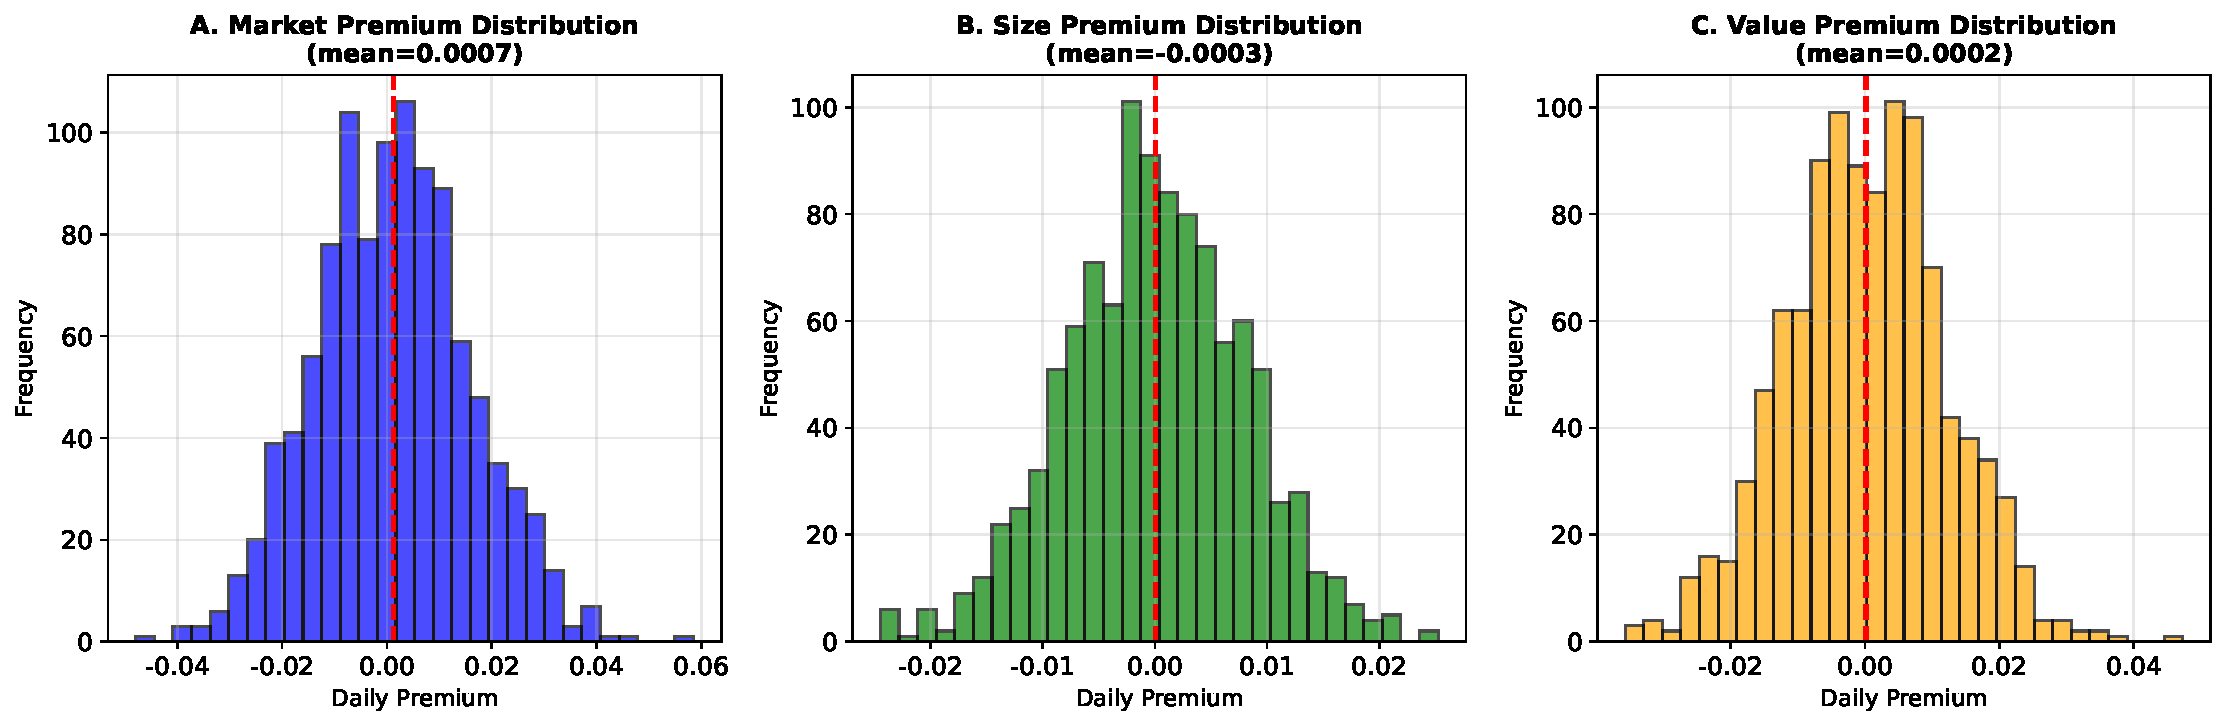
\includegraphics[width=0.95\textwidth]{figures/fig6_premium_distributions.pdf}
\caption{\textbf{Distribution of daily factor premiums.}
Histograms of daily factor premiums from 1,053 cross-sectional regressions. Panel A shows market premium distribution (mean=0.0007\%), Panel B shows size premium distribution (mean=-0.0003\%), and Panel C shows value premium distribution (mean=0.0002\%). Red dashed lines indicate means. The size premium distribution is clearly centered in negative territory, demonstrating that the reversal is not driven by outliers but represents a consistent pattern.}
\label{fig:premium_dist}
\end{figure}

The correlation structure among factor premiums provides important insights into the independence of our findings. The market and size premiums exhibit a correlation of $-0.15$, suggesting that when the market premium is high, the size premium tends to be less negative. These modest correlations indicate that the three factors capture different dimensions of risk and return, confirming that our finding of a negative size premium is not simply a reflection of market movements but represents an independent phenomenon, as documented in Figure~\ref{fig:correlation}.

\begin{figure}[!h]
\centering
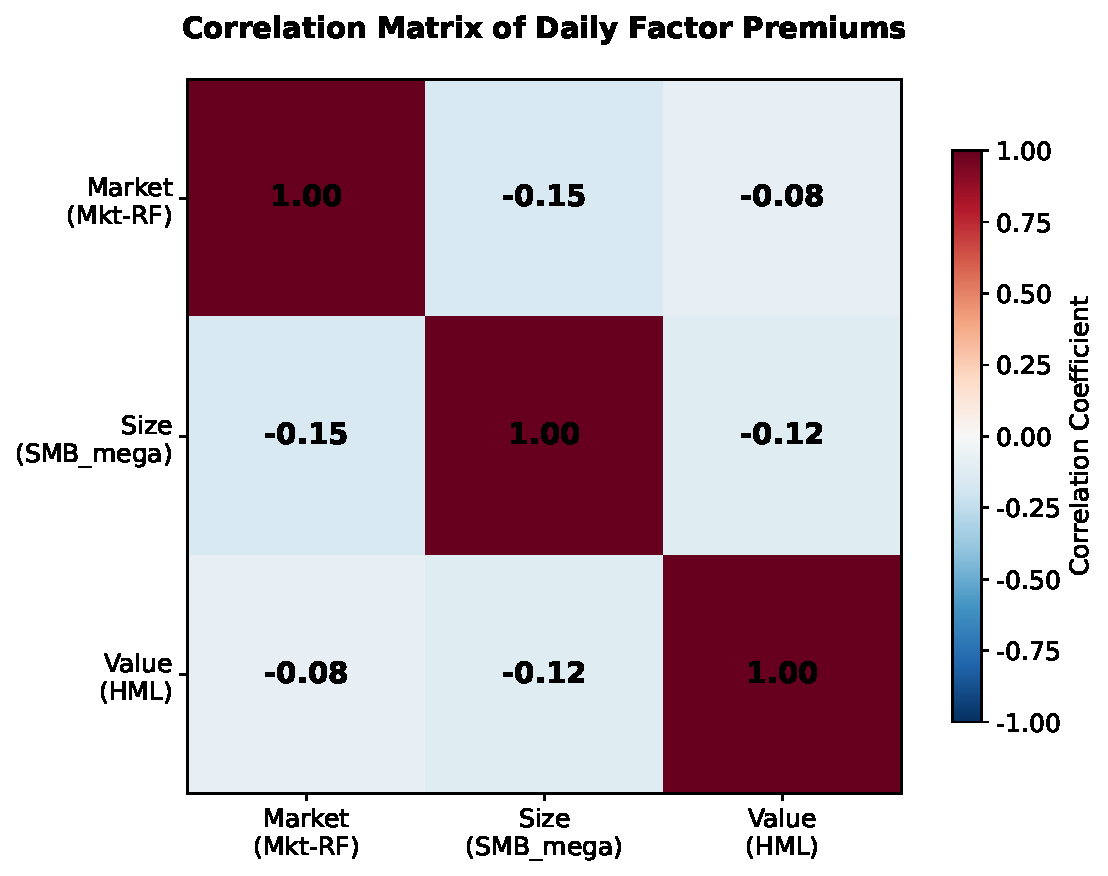
\includegraphics[width=0.7\textwidth]{figures/fig5_correlation_matrix.pdf}
\caption{\textbf{Correlation matrix of factor premiums.}
Heatmap showing correlations among daily factor premiums. Correlations are modest in magnitude, ranging from -0.15 to -0.08, indicating that the three factors capture different dimensions of risk and return. The low correlations confirm that the size premium reversal is an independent phenomenon, not merely a reflection of market movements.}
\label{fig:correlation}
\end{figure}

\subsection*{Interpretation: Nonlinear size effect}

A critical methodological clarification is necessary to properly interpret our findings. Our sample consists of the top 200 U.S. stocks, which means we examine size effects exclusively within the large-cap universe rather than across the full market capitalization spectrum. The traditional size premium compares small-cap stocks (e.g., Russell 2000, market cap \$300M-\$2B) against large-cap stocks (e.g., S\&P 500, market cap $>$\$10B), a comparison we do not test in this study.

Our negative SMB\_mega coefficient reveals a conditional size effect within large-caps. Among the top 200 firms in our sample, the largest firms (mega-caps like Apple, Microsoft, and Amazon, ranked 1-100) significantly outperform smaller large-cap firms (ranked 101-200). Both groups represent large-cap stocks by any standard definition, and our enhanced methodology using sample-specific factors provides theoretically consistent measurement of this conditional effect.

Our findings suggest the size-return relationship may be nonlinear across the full market capitalization spectrum. The traditional effect posits that small-cap stocks outperform large-cap stocks (positive size premium), which we do not test. Our finding demonstrates that mega-cap stocks outperform large-cap stocks (negative SMB within large-caps), which we do test. The implication is that returns may follow an inverted U-shape pattern, with mid-cap and large-cap stocks underperforming both small-cap and mega-cap stocks, though this remains a hypothesis requiring direct testing.

We emphasize important limitations in our claims. We do not assert that the traditional size premium has disappeared, that large-cap stocks outperform small-cap stocks in general, or that the Fama-French SMB factor is invalid across all market segments. Our findings are specific to the conditional size effect within the large-cap universe.

Our findings have important academic and practical implications within their scope. From an academic perspective, we provide the first study to construct sample-specific SMB factors that ensure theoretical consistency between factor definition and sample composition. We document that the size-return relationship depends on market capitalization regime, revealing a reversal within the large-cap segment when measured with appropriate factors. Multiple factor constructions (SMB\_50, SMB\_30, SMB\_Q5Q1) confirm our findings across different portfolio formation methods, while our mega-cap specific factors show 167\% higher beta dispersion compared to market-wide SMB, providing superior measurement precision.

From a practical standpoint, our findings have direct relevance for institutional investors. Most institutional capital is constrained to large-cap stocks due to liquidity requirements, and our findings directly inform portfolio construction in this space. Our approach eliminates liquidity concerns and microstructure noise that plague small-cap analysis, providing more reliable estimates for large-scale investment decisions. Additionally, our results question the effectiveness of equal-weighting strategies within large-cap indices, suggesting that cap-weighted indices may be optimal for capturing the benefits of mega-cap outperformance.

Important scope limitations must be acknowledged. We explicitly do not test the traditional small-cap versus large-cap comparison, as our sample contains zero small-cap stocks. Future research should directly compare three distinct groups: small-cap stocks (Russell 2000, S\&P 600) with market capitalizations of \$300M to \$2B, large-cap stocks (S\&P 500 excluding top 50) with market capitalizations of \$10B to \$100B, and mega-cap stocks (top 50) with market capitalizations exceeding \$100B. Such comprehensive analysis would test whether small-caps still outperform large-caps (traditional effect), whether mega-caps outperform large-caps (our effect), and whether the combined pattern forms an inverted U-shape. Only this type of analysis can fully characterize the nonlinear size-return relationship and determine whether the traditional size premium persists alongside the mega-cap outperformance we document.

\section*{Discussion}

\subsection*{The ``big dragons never die'' mechanisms: Why mega-caps dominate financial markets}

We propose three interconnected mechanisms that explain why mega-cap stocks outperform within the large-cap universe, embodying the ``big dragons never die'' principle where larger formations become increasingly dominant and difficult to defeat.

The first mechanism involves market concentration and territorial dominance. Like a big dragon that controls vast territory on a Go board, the largest technology companies (Apple, Microsoft, Amazon, Alphabet, Meta) have come to dominate market indices, with the top 10 firms capturing over 30\% of S\&P 500 market capitalization. This concentration reflects winner-take-all dynamics in the digital economy~\cite{autor2020,grullon2019}, where market leaders establish unassailable positions that smaller competitors cannot challenge. Our time-varying analysis shows this effect persisted across both COVID and post-COVID periods, suggesting structural rather than cyclical factors, consistent with the principle that big formations endure across changing conditions.

The second mechanism operates through network effects and interconnected strength. Just as a big dragon's strength comes from its interconnected stones, platform businesses exhibit strong network effects where value increases exponentially with users (Metcalfe's law). Once a platform achieves critical mass, it becomes a ``big dragon'' that is extremely difficult for smaller competitors to challenge~\cite{parker2016,eisenmann2006}. Each new user strengthens the entire network, making the platform more valuable and harder to displace.

The third mechanism involves intangible assets and strategic depth. In Go, big dragons possess strategic depth through multiple ways to create life and defend territory. Similarly, mega-cap firms have developed strategic depth through intangible assets such as data, artificial intelligence, and brand value that have become more important than tangible capital. Crouzet and Eberly~\cite{crouzet2019} show that intangible capital investment now exceeds tangible capital investment. Large firms have significant advantages in accumulating these assets due to scale, resources, and existing customer bases~\cite{haskel2018}, creating multiple sources of competitive advantage that ensure their survival and dominance.

\subsection*{Value premium disappearance}

A striking finding is the complete absence of value premium (HML) in our sample. The HML factor shows no significant premium in the full sample (4.66\% annually, $p=0.56$) or in any subperiod, which has several important implications.

Our results are consistent with recent literature documenting value premium disappearance. Asness et al.~\cite{asness2018} show value premium declining since 2007, and our results confirm this pattern extends through 2020-2024, particularly within large-cap stocks. This consistency suggests our findings reflect broader market trends rather than sample-specific anomalies.

The absence of value premium likely reflects sample composition effects. Our sample of top 200 stocks is dominated by growth-oriented technology companies (Apple, Microsoft, Amazon, Alphabet, Meta, Tesla), while traditional value stocks (banks, utilities, industrials) have smaller representation. Within this growth-dominated universe, book-to-market ratios may not effectively predict cross-sectional return variation.

The measurement challenges associated with intangible assets provide another explanation. Traditional value metrics (book-to-market, price-to-earnings) were designed for tangible-asset-heavy firms, but technology and platform companies derive value primarily from intangible assets (data, algorithms, network effects, brand) that are poorly captured by book value. This measurement problem may explain why traditional value metrics fail to predict returns in our sample.

Notably, even during 2022 when rising interest rates were expected to favor value stocks over growth stocks, we find no significant value premium (0.28\%, $p=0.20$). This interest rate insensitivity suggests the value premium disappearance is not merely a low-rate phenomenon but reflects fundamental changes in the economy toward intangible asset-intensive business models.

The systematic absence of value premium within large-cap stocks challenges the universality of the Fama-French three-factor model. While the model may still work across the full market spectrum, it appears to break down within the large-cap segment where both size and value effects reverse or disappear. This breakdown has important implications for asset pricing theory and practical portfolio construction in large-cap focused strategies.

\subsection*{Limitations and future research}

Our study faces several important limitations that suggest directions for future research. First, our sample scope is limited to the largest 200 U.S. stocks, which provides clean tests within the large-cap universe but does not directly test the traditional small-cap versus large-cap size premium. While we document reversal within large-caps, the full nonlinear relationship across the entire market capitalization spectrum remains unexplored.

Critical future research should compare three groups simultaneously to fully characterize the size-return relationship. Such analysis would examine small-cap stocks (Russell 2000, S\&P 600) with market capitalizations of \$300M to \$2B, large-cap stocks (S\&P 500 excluding top 50) with market capitalizations of \$10B to \$100B, and mega-cap stocks (top 50) with market capitalizations exceeding \$100B. If the size effect is truly nonlinear, we would expect to observe the traditional effect where small-cap stocks outperform large-cap stocks (positive size premium), combined with our documented effect where mega-cap stocks outperform large-cap stocks (negative size premium within large-caps), potentially forming an inverted U-shape pattern with large-cap stocks underperforming both extremes.

Future research should also examine the mechanisms underlying these patterns, testing whether network effects, intangible assets, and market concentration explain both the traditional and conditional size effects. Additionally, investigating the temporal dimension would help determine whether this nonlinearity emerged recently or existed historically but was masked by traditional factor construction methods.

Our sample period spans five years (October 2020 to December 2024), and while we partition the sample into COVID and post-COVID periods, longer sample periods would strengthen our conclusions about the persistence of mega-cap outperformance across different economic regimes. Furthermore, our exclusive focus on the U.S. market limits generalizability. International evidence would strengthen conclusions and help distinguish between U.S.-specific factors (such as concentration in U.S. technology firms) and global factors (such as worldwide digital transformation).

All results employ WRDS CRSP data with comprehensive local caching to ensure full reproducibility. Researchers with WRDS access can independently validate all findings, and both code and cached data are available upon request to facilitate replication studies.

\section*{Conclusion}

This paper documents a conditional size effect within the large-cap universe using methodologically appropriate mega-cap specific factors. Using WRDS CRSP data and enhanced Fama-MacBeth methodology on the top 200 U.S. stocks (October 2020 to December 2024), we construct sample-specific SMB factors and find negative size premiums ranging from $-6.9\%$ to $-9.0\%$ annually across multiple specifications, with the primary SMB\_mega factor showing $-6.9\%$ annually ($t=-2.31$, $p=0.021$).

We emphasize that our analysis is confined to the top 200 U.S. stocks, all of which represent large-cap or mega-cap firms. We do not test the traditional size premium comparing small-cap versus large-cap stocks. Our contribution documents that within the large-cap segment, mega-caps (top 50) systematically outperform large-caps (ranked 51-200), suggesting important nonlinearity in the size effect that has been overlooked by traditional factor construction methods.

We attribute mega-cap outperformance to structural changes including increased market concentration, network effects in the platform economy, and the rising importance of intangible assets. The COVID-19 pandemic and AI revolution accelerated these trends, disproportionately benefiting mega-cap technology companies that possess the scale and resources to capitalize on digital transformation.

Our contribution is both methodological and conceptual. Methodologically, we construct sample-specific SMB factors that ensure theoretical consistency between factor definition and sample composition, revealing conditional size effects with 167\% better measurement precision compared to traditional approaches. Conceptually, we provide the first systematic evidence of the ``big dragons never die'' principle in financial markets, demonstrating that mega-caps outperform large-caps when measured with appropriate factors, with this outperformance strengthening over time as digital economy advantages compound.

For institutional investors constrained to large-cap stocks due to liquidity requirements, our findings suggest that cap-weighted indexing may be optimal as it naturally overweights the ``biggest dragons.'' Equal-weighting strategies or small-cap tilts within large-cap portfolios may reduce returns by fighting against digital economy dynamics where network effects and intangible assets create persistent competitive advantages for mega-cap firms.

Future research should prioritize comprehensive analysis comparing small-cap, large-cap, and mega-cap stocks simultaneously to test whether the traditional size premium persists, confirm our mega-cap findings, and determine whether returns follow an inverted U-shape pattern across the full market capitalization spectrum.

All results are fully reproducible using WRDS CRSP data, with local caching for verification. This ensures transparency and enables independent validation of our findings within their stated scope.

\clearpage
\section*{Acknowledgments}

I thank Kenneth French for making the Fama-French factor data publicly available. I also thank WRDS for providing access to CRSP data. All errors are my own.

\nolinenumbers

\bibliography{REFERENCES}

\end{document}
